%----------------------------------------------------------------------------------------
%	PACKAGES AND OTHER DOCUMENT CONFIGURATIONS
%----------------------------------------------------------------------------------------

\documentclass[11pt,fleqn]{book} % Default font size and left-justified equations

\usepackage[top=3cm,bottom=3cm,left=3.2cm,right=3.2cm,headsep=10pt,letterpaper]{geometry} % Page margins
\usepackage{tikz}
\usepackage{xcolor}
\definecolor{ocre}{RGB}{52,177,201}

% Font Settings
\usepackage{avant}
\usepackage{mathptmx}
\usepackage{microtype}
\usepackage[utf8]{inputenc}
\usepackage[T1]{fontenc}

% Bibliography
\usepackage[style=alphabetic,sorting=nyt,sortcites=true,autopunct=true,babel=hyphen,hyperref=true,abbreviate=false,backref=true,backend=biber]{biblatex}
\addbibresource{bibliography.bib} % BibTeX bibliography file
\defbibheading{bibempty}{}

%----------------------------------------------------------------------------------------
%	VARIOUS REQUIRED PACKAGES
%----------------------------------------------------------------------------------------

\usepackage{titlesec} % Allows customization of titles

\usepackage{graphicx} % Required for including pictures
\graphicspath{{Pictures/}} % Specifies the directory where pictures are stored

\usepackage{lipsum} % Inserts dummy text

\usepackage{tikz} % Required for drawing custom shapes

\usepackage[english]{babel} % English language/hyphenation

\usepackage{enumitem} % Customize lists
\setlist{nolistsep} % Reduce spacing between bullet points and numbered lists

\usepackage{booktabs} % Required for nicer horizontal rules in tables

\usepackage{eso-pic} % Required for specifying an image background in the title page

%----------------------------------------------------------------------------------------
%	MAIN TABLE OF CONTENTS
%----------------------------------------------------------------------------------------

\usepackage{titletoc} % Required for manipulating the table of contents

\contentsmargin{0cm} % Removes the default margin
% Chapter text styling
\titlecontents{chapter}[1.25cm] % Indentation
{\addvspace{15pt}\large\sffamily\bfseries} % Spacing and font options for chapters
{\color{ocre!60}\contentslabel[\Large\thecontentslabel]{1.25cm}\color{ocre}} % Chapter number
{}  
{\color{ocre!60}\normalsize\sffamily\bfseries\;\titlerule*[.5pc]{.}\;\thecontentspage} % Page number
% Section text styling
\titlecontents{section}[1.25cm] % Indentation
{\addvspace{5pt}\sffamily\bfseries} % Spacing and font options for sections
{\contentslabel[\thecontentslabel]{1.25cm}} % Section number
{}
{\sffamily\hfill\color{black}\thecontentspage} % Page number
[]
% Subsection text styling
\titlecontents{subsection}[1.25cm] % Indentation
{\addvspace{1pt}\sffamily\small} % Spacing and font options for subsections
{\contentslabel[\thecontentslabel]{1.25cm}} % Subsection number
{}
{\sffamily\;\titlerule*[.5pc]{.}\;\thecontentspage} % Page number
[] 

%----------------------------------------------------------------------------------------
%	MINI TABLE OF CONTENTS IN CHAPTER HEADS
%----------------------------------------------------------------------------------------

% Section text styling
\titlecontents{lsection}[0em] % Indendating
{\footnotesize\sffamily} % Font settings
{}
{}
{}

% Subsection text styling
\titlecontents{lsubsection}[.5em] % Indentation
{\normalfont\footnotesize\sffamily} % Font settings
{}
{}
{}
 
%----------------------------------------------------------------------------------------
%	PAGE HEADERS
%----------------------------------------------------------------------------------------

\usepackage{fancyhdr} % Required for header and footer configuration

\pagestyle{fancy}
\renewcommand{\chaptermark}[1]{\markboth{\sffamily\normalsize\bfseries\chaptername\ \thechapter.\ #1}{}} % Chapter text font settings
\renewcommand{\sectionmark}[1]{\markright{\sffamily\normalsize\thesection\hspace{5pt}#1}{}} % Section text font settings
\fancyhf{} \fancyhead[LE,RO]{\sffamily\normalsize\thepage} % Font setting for the page number in the header
\fancyhead[LO]{\rightmark} % Print the nearest section name on the left side of odd pages
\fancyhead[RE]{\leftmark} % Print the current chapter name on the right side of even pages
\renewcommand{\headrulewidth}{0.5pt} % Width of the rule under the header
\addtolength{\headheight}{2.5pt} % Increase the spacing around the header slightly
\renewcommand{\footrulewidth}{0pt} % Removes the rule in the footer
\fancypagestyle{plain}{\fancyhead{}\renewcommand{\headrulewidth}{0pt}} % Style for when a plain pagestyle is specified

% Removes the header from odd empty pages at the end of chapters
\makeatletter
\renewcommand{\cleardoublepage}{
\clearpage\ifodd\c@page\else
\hbox{}
\vspace*{\fill}
\thispagestyle{empty}
\newpage
\fi}

%----------------------------------------------------------------------------------------
%	THEOREM STYLES
%----------------------------------------------------------------------------------------

\usepackage{amsmath,amsfonts,amssymb,amsthm} % For math equations, theorems, symbols, etc

\newcommand{\intoo}[2]{\mathopen{]}#1\,;#2\mathclose{[}}
\newcommand{\ud}{\mathop{\mathrm{{}d}}\mathopen{}}
\newcommand{\intff}[2]{\mathopen{[}#1\,;#2\mathclose{]}}
\newtheorem{notation}{Notation}[chapter]

%%%%%%%%%%%%%%%%%%%%%%%%%%%%%%%%%%%%%%%%%%%%%%%%%%%%%%%%%%%%%%%%%%%%%%%%%%%
%%%%%%%%%%%%%%%%%%%% dedicated to boxed/framed environements %%%%%%%%%%%%%%
%%%%%%%%%%%%%%%%%%%%%%%%%%%%%%%%%%%%%%%%%%%%%%%%%%%%%%%%%%%%%%%%%%%%%%%%%%%
\newtheoremstyle{ocrenumbox}% % Theorem style name
{0pt}% Space above
{0pt}% Space below
{\normalfont}% % Body font
{}% Indent amount
{\small\bf\sffamily\color{ocre}}% % Theorem head font
{\;}% Punctuation after theorem head
{0.25em}% Space after theorem head
{\small\sffamily\color{ocre}\thmname{#1}\nobreakspace\thmnumber{\@ifnotempty{#1}{}\@upn{#2}}% Theorem text (e.g. Theorem 2.1)
\thmnote{\nobreakspace\the\thm@notefont\sffamily\bfseries\color{black}---\nobreakspace#3.}} % Optional theorem note
\renewcommand{\qedsymbol}{$\blacksquare$}% Optional qed square

\newtheoremstyle{blacknumex}% Theorem style name
{5pt}% Space above
{5pt}% Space below
{\normalfont}% Body font
{} % Indent amount
{\small\bf\sffamily}% Theorem head font
{\;}% Punctuation after theorem head
{0.25em}% Space after theorem head
{\small\sffamily{\tiny\ensuremath{\blacksquare}}\nobreakspace\thmname{#1}\nobreakspace\thmnumber{\@ifnotempty{#1}{}\@upn{#2}}% Theorem text (e.g. Theorem 2.1)
\thmnote{\nobreakspace\the\thm@notefont\sffamily\bfseries---\nobreakspace#3.}}% Optional theorem note

\newtheoremstyle{blacknumbox} % Theorem style name
{0pt}% Space above
{0pt}% Space below
{\normalfont}% Body font
{}% Indent amount
{\small\bf\sffamily}% Theorem head font
{\;}% Punctuation after theorem head
{0.25em}% Space after theorem head
{\small\sffamily\thmname{#1}\nobreakspace\thmnumber{\@ifnotempty{#1}{}\@upn{#2}}% Theorem text (e.g. Theorem 2.1)
\thmnote{\nobreakspace\the\thm@notefont\sffamily\bfseries---\nobreakspace#3.}}% Optional theorem note

%%%%%%%%%%%%%%%%%%%%%%%%%%%%%%%%%%%%%%%%%%%%%%%%%%%%%%%%%%%%%%%%%%%%%%%%%%%
%%%%%%%%%%%%% dedicated to non-boxed/non-framed environements %%%%%%%%%%%%%
%%%%%%%%%%%%%%%%%%%%%%%%%%%%%%%%%%%%%%%%%%%%%%%%%%%%%%%%%%%%%%%%%%%%%%%%%%%
\newtheoremstyle{ocrenum}% % Theorem style name
{5pt}% Space above
{5pt}% Space below
{\normalfont}% % Body font
{}% Indent amount
{\small\bf\sffamily\color{ocre}}% % Theorem head font
{\;}% Punctuation after theorem head
{0.25em}% Space after theorem head
{\small\sffamily\color{ocre}\thmname{#1}\nobreakspace\thmnumber{\@ifnotempty{#1}{}\@upn{#2}}% Theorem text (e.g. Theorem 2.1)
\thmnote{\nobreakspace\the\thm@notefont\sffamily\bfseries\color{black}---\nobreakspace#3.}} % Optional theorem note
\renewcommand{\qedsymbol}{$\blacksquare$}% Optional qed square
\makeatother

% Defines the theorem text style for each type of theorem to one of the three styles above
\newcounter{dummy} 
\numberwithin{dummy}{section}
\theoremstyle{ocrenumbox}
\newtheorem{theoremeT}[dummy]{Theorem}
\newtheorem{problem}{Problem}[chapter]
\newtheorem{exerciseT}{Exercise}[chapter]
\theoremstyle{blacknumex}
\newtheorem{exampleT}{Example}[chapter]
\theoremstyle{blacknumbox}
\newtheorem{vocabulary}{Vocabulary}[chapter]
\newtheorem{definitionT}{Definition}[section]
\newtheorem{corollaryT}[dummy]{Corollary}
\theoremstyle{ocrenum}
\newtheorem{proposition}[dummy]{Proposition}

%----------------------------------------------------------------------------------------
%	DEFINITION OF COLORED BOXES
%----------------------------------------------------------------------------------------

\RequirePackage[framemethod=default]{mdframed} % Required for creating the theorem, definition, exercise and corollary boxes

% Theorem box
\newmdenv[skipabove=7pt,
skipbelow=7pt,
backgroundcolor=black!5,
linecolor=ocre,
innerleftmargin=5pt,
innerrightmargin=5pt,
innertopmargin=5pt,
leftmargin=0cm,
rightmargin=0cm,
innerbottommargin=5pt]{tBox}

% Exercise box	  
\newmdenv[skipabove=7pt,
skipbelow=7pt,
rightline=false,
leftline=true,
topline=false,
bottomline=false,
backgroundcolor=ocre!10,
linecolor=ocre,
innerleftmargin=5pt,
innerrightmargin=5pt,
innertopmargin=5pt,
innerbottommargin=5pt,
leftmargin=0cm,
rightmargin=0cm,
linewidth=4pt]{eBox}	

% Definition box
\newmdenv[skipabove=7pt,
skipbelow=7pt,
rightline=false,
leftline=true,
topline=false,
bottomline=false,
linecolor=ocre,
innerleftmargin=5pt,
innerrightmargin=5pt,
innertopmargin=0pt,
leftmargin=0cm,
rightmargin=0cm,
linewidth=4pt,
innerbottommargin=0pt]{dBox}	

% Corollary box
\newmdenv[skipabove=7pt,
skipbelow=7pt,
rightline=false,
leftline=true,
topline=false,
bottomline=false,
linecolor=gray,
backgroundcolor=black!5,
innerleftmargin=5pt,
innerrightmargin=5pt,
innertopmargin=5pt,
leftmargin=0cm,
rightmargin=0cm,
linewidth=4pt,
innerbottommargin=5pt]{cBox}

% Creates an environment for each type of theorem and assigns it a theorem text style from the "Theorem Styles" section above and a colored box from above
\newenvironment{theorem}{\begin{tBox}\begin{theoremeT}}{\end{theoremeT}\end{tBox}}
\newenvironment{exercise}{\begin{eBox}\begin{exerciseT}}{\hfill{\color{ocre}\tiny\ensuremath{\blacksquare}}\end{exerciseT}\end{eBox}}				  
\newenvironment{definition}{\begin{dBox}\begin{definitionT}}{\end{definitionT}\end{dBox}}	
\newenvironment{example}{\begin{exampleT}}{\hfill{\tiny\ensuremath{\blacksquare}}\end{exampleT}}		
\newenvironment{corollary}{\begin{cBox}\begin{corollaryT}}{\end{corollaryT}\end{cBox}}	

%----------------------------------------------------------------------------------------
%	REMARK ENVIRONMENT
%----------------------------------------------------------------------------------------

\newenvironment{remark}{\par\vspace{10pt}\small % Vertical white space above the remark and smaller font size
\begin{list}{}{
\leftmargin=35pt % Indentation on the left
\rightmargin=25pt}\item\ignorespaces % Indentation on the right
\makebox[-2.5pt]{\begin{tikzpicture}[overlay]
\node[draw=ocre!60,line width=1pt,circle,fill=ocre!25,font=\sffamily\bfseries,inner sep=2pt,outer sep=0pt] at (-15pt,0pt){\textcolor{ocre}{R}};\end{tikzpicture}} % Orange R in a circle
\advance\baselineskip -1pt}{\end{list}\vskip5pt} % Tighter line spacing and white space after remark

%----------------------------------------------------------------------------------------
%	SECTION NUMBERING IN THE MARGIN
%----------------------------------------------------------------------------------------

\makeatletter
\renewcommand{\@seccntformat}[1]{\llap{\textcolor{ocre}{\csname the#1\endcsname}\hspace{1em}}}                    
\renewcommand{\section}{\@startsection{section}{1}{\z@}
{-4ex \@plus -1ex \@minus -.4ex}
{1ex \@plus.2ex }
{\normalfont\large\sffamily\bfseries}}
\renewcommand{\subsection}{\@startsection {subsection}{2}{\z@}
{-3ex \@plus -0.1ex \@minus -.4ex}
{0.5ex \@plus.2ex }
{\normalfont\sffamily\bfseries}}
\renewcommand{\subsubsection}{\@startsection {subsubsection}{3}{\z@}
{-2ex \@plus -0.1ex \@minus -.2ex}
{.2ex \@plus.2ex }
{\normalfont\small\sffamily\bfseries}}                        
\renewcommand\paragraph{\@startsection{paragraph}{4}{\z@}
{-2ex \@plus-.2ex \@minus .2ex}
{.1ex}
{\normalfont\small\sffamily\bfseries}}

%----------------------------------------------------------------------------------------
%	HYPERLINKS IN THE DOCUMENTS
%----------------------------------------------------------------------------------------

% For an unclear reason, the package should be loaded now and not later
\usepackage{hyperref}
\hypersetup{hidelinks,backref=true,pagebackref=true,hyperindex=true,colorlinks=false,breaklinks=true,urlcolor= ocre,bookmarks=true,bookmarksopen=false,pdftitle={Title},pdfauthor={Author}}

%----------------------------------------------------------------------------------------
%	CHAPTER HEADINGS
%----------------------------------------------------------------------------------------

% The set-up below should be (sadly) manually adapted to the overall margin page septup controlled by the geometry package loaded in the main.tex document. It is possible to implement below the dimensions used in the goemetry package (top,bottom,left,right)... TO BE DONE

\newcommand{\thechapterimage}{}
\newcommand{\chapterimage}[1]{\renewcommand{\thechapterimage}{#1}}

% Numbered chapters with mini tableofcontents
\def\thechapter{\arabic{chapter}}
\def\@makechapterhead#1{
\thispagestyle{empty}
{\centering \normalfont\sffamily
\ifnum \c@secnumdepth >\m@ne
\if@mainmatter
\startcontents
\begin{tikzpicture}[remember picture,overlay]
\node at (current page.north west)
{\begin{tikzpicture}[remember picture,overlay]
\node[anchor=north west,inner sep=0pt] at (0,0) {\includegraphics[width=\paperwidth]{\thechapterimage}};
%%%%%%%%%%%%%%%%%%%%%%%%%%%%%%%%%%%%%%%%%%%%%%%%%%%%%%%%%%%%%%%%%%%%%%%%%%%%%%%%%%%%%
% Commenting the 3 lines below removes the small contents box in the chapter heading
%\fill[color=ocre!10!white,opacity=.6] (1cm,0) rectangle (8cm,-7cm);
%\node[anchor=north west] at (1.1cm,.35cm) {\parbox[t][8cm][t]{6.5cm}{\huge\bfseries\flushleft \printcontents{l}{1}{\setcounter{tocdepth}{2}}}};
\draw[anchor=west] (5cm,-9cm) node [rounded corners=20pt,fill=ocre!10!white,text opacity=1,draw=ocre,draw opacity=1,line width=1.5pt,fill opacity=.6,inner sep=12pt]{\huge\sffamily\bfseries\textcolor{black}{\thechapter. #1\strut\makebox[22cm]{}}};
%%%%%%%%%%%%%%%%%%%%%%%%%%%%%%%%%%%%%%%%%%%%%%%%%%%%%%%%%%%%%%%%%%%%%%%%%%%%%%%%%%%%%
\end{tikzpicture}};
\end{tikzpicture}}
\par\vspace*{230\p@}
\fi
\fi}

% Unnumbered chapters without mini tableofcontents (could be added though) 
\def\@makeschapterhead#1{
\thispagestyle{empty}
{\centering \normalfont\sffamily
\ifnum \c@secnumdepth >\m@ne
\if@mainmatter
\begin{tikzpicture}[remember picture,overlay]
\node at (current page.north west)
{\begin{tikzpicture}[remember picture,overlay]
\node[anchor=north west,inner sep=0pt] at (0,0) {\includegraphics[width=\paperwidth]{\thechapterimage}};
\draw[anchor=west] (5cm,-9cm) node [rounded corners=20pt,fill=ocre!10!white,fill opacity=.6,inner sep=12pt,text opacity=1,draw=ocre,draw opacity=1,line width=1.5pt]{\huge\sffamily\bfseries\textcolor{black}{#1\strut\makebox[22cm]{}}};
\end{tikzpicture}};
\end{tikzpicture}}
\par\vspace*{230\p@}
\fi
\fi
}
\makeatother 
\begin{document}

%----------------------------------------------------------------------------------------
%	TITLE PAGE
%----------------------------------------------------------------------------------------
\begingroup
\thispagestyle{empty}
\AddToShipoutPicture*{\put(0,0){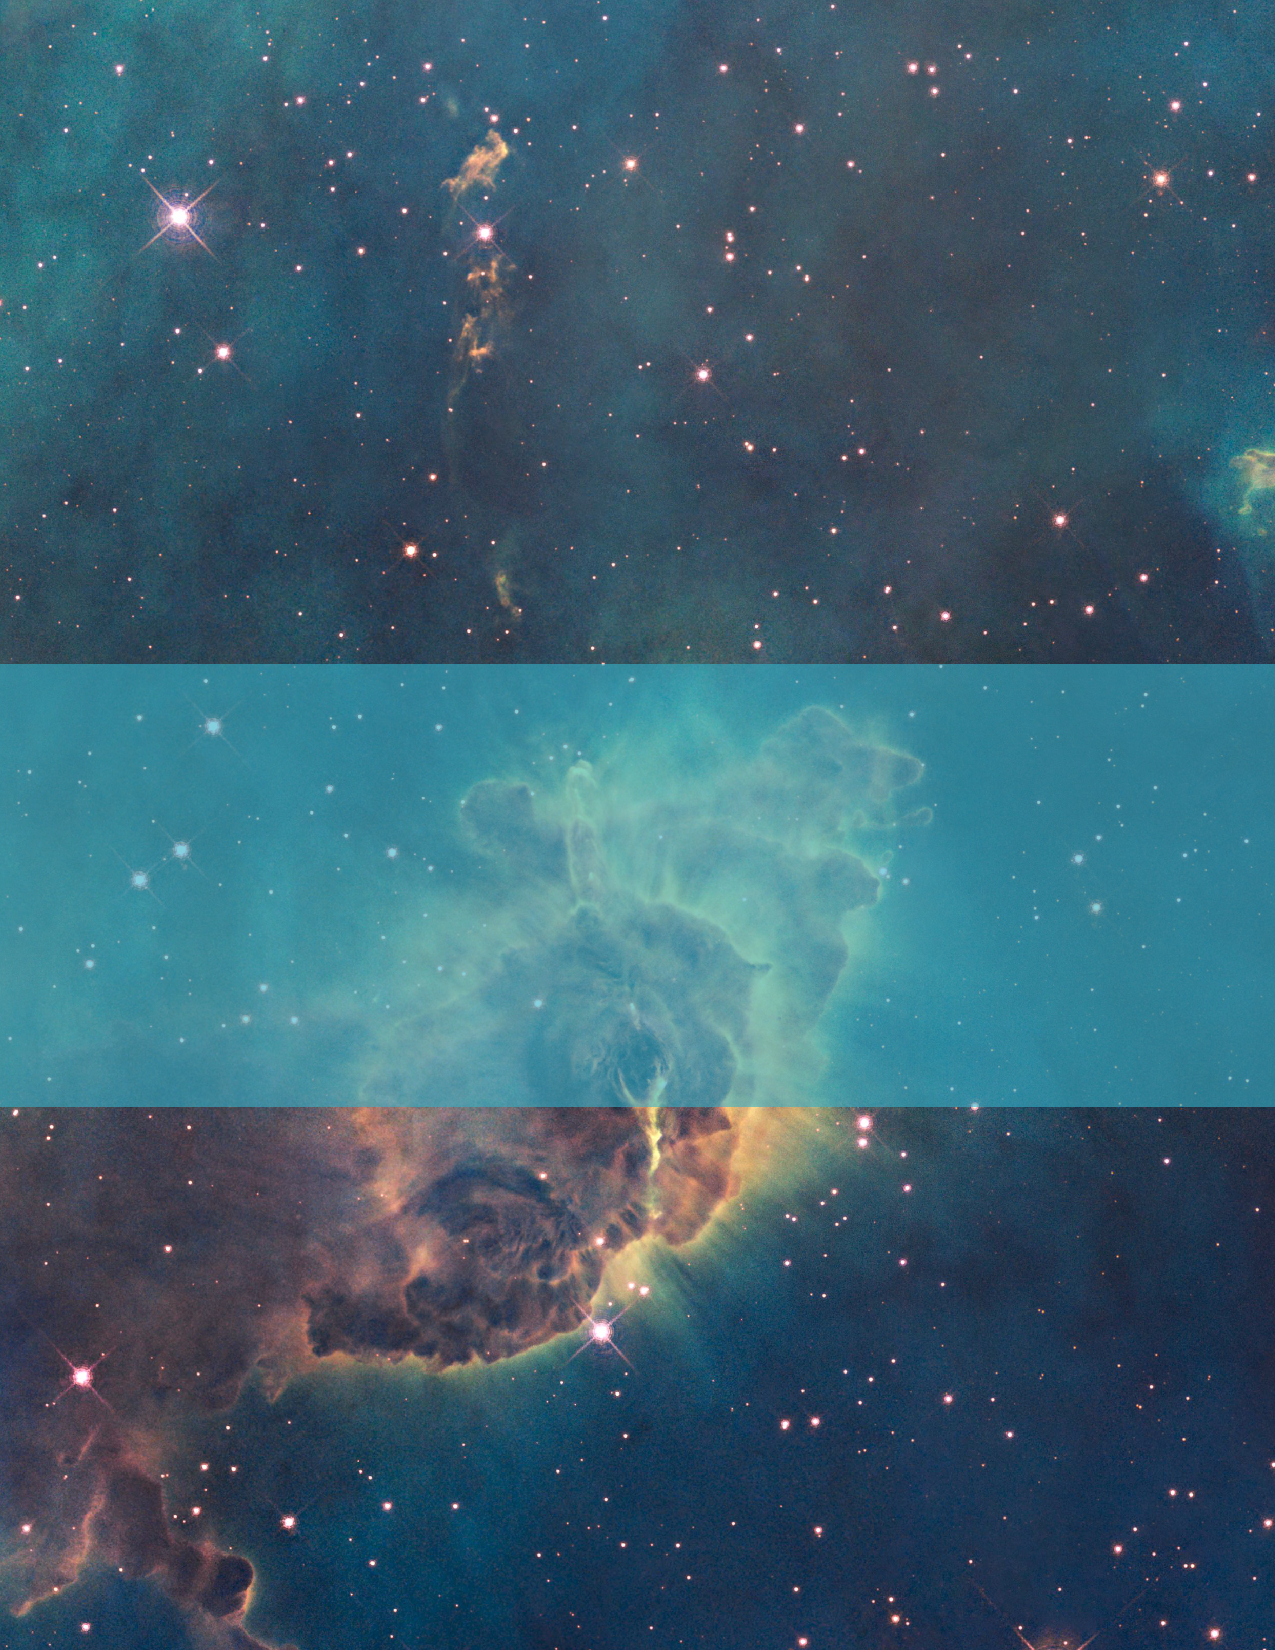
\includegraphics[scale=1.25]{esahubble}}} % Image background
\centering
\vspace*{5cm}
\par\normalfont\fontsize{35}{35}\sffamily\selectfont
\textbf{Aut\'omatas Deterministicos de Estados Finitos}\\
{\LARGE Commpiladores e Int\'ertpretes\\Tecnol\'ogico de Costa Rica}\par % Book title
\vspace*{0.5cm}
{\Huge Samantha Arburola Le\'on}\par 
\endgroup
%----------------------------------------------------------------------------------------
\newpage
\section{Automaton 12}
The set of strings over \{a,b,c\} in which all the a's precede the b's, which in turn procede the c's. It is possible that there are no a's, b's or c's.\\
{\sc Solution}\\
\begin{center}
\begin{tikzpicture}[scale=0.2]
\tikzstyle{every node}+=[inner sep=0pt]
\draw [black] (12.9,-24.8) circle (3);
\draw (12.9,-24.8) node {$Q_0$};
\draw [black] (12.9,-24.8) circle (2.4);
\draw [black] (25.7,-24.8) circle (3);
\draw (25.7,-24.8) node {$Q_1$};
\draw [black] (25.7,-24.8) circle (2.4);
\draw [black] (40.2,-24.8) circle (3);
\draw (40.2,-24.8) node {$Q_2$};
\draw [black] (40.2,-24.8) circle (2.4);
\draw [black] (55.9,-24.8) circle (3);
\draw (55.9,-24.8) node {$Q_3$};
\draw [black] (55.9,-24.8) circle (2.4);
\draw [black] (7.7,-20.1) -- (10.67,-22.79);
\fill [black] (10.67,-22.79) -- (10.42,-21.88) -- (9.75,-22.62);
\draw [black] (28.7,-24.8) -- (37.2,-24.8);
\fill [black] (37.2,-24.8) -- (36.4,-24.3) -- (36.4,-25.3);
\draw (32.95,-25.3) node [below] {$b$};
\draw [black] (15.9,-24.8) -- (22.7,-24.8);
\fill [black] (22.7,-24.8) -- (21.9,-24.3) -- (21.9,-25.3);
\draw (19.3,-25.3) node [below] {$a$};
\draw [black] (43.2,-24.8) -- (52.9,-24.8);
\fill [black] (52.9,-24.8) -- (52.1,-24.3) -- (52.1,-25.3);
\draw (48.05,-25.3) node [below] {$c$};
\draw [black] (15.264,-22.958) arc (123.70089:56.29911:20.34);
\fill [black] (37.84,-22.96) -- (37.45,-22.1) -- (36.89,-22.93);
\draw (26.55,-19.04) node [above] {$b$};
\draw [black] (15.031,-22.69) arc (131.76445:48.23555:29.08);
\fill [black] (53.77,-22.69) -- (53.51,-21.78) -- (52.84,-22.53);
\draw (34.4,-14.8) node [above] {$c$};
\draw [black] (25.455,-27.778) arc (23.03624:-264.96376:2.25);
\draw (21.13,-31.09) node [below] {$a$};
\fill [black] (23.19,-26.42) -- (22.26,-26.27) -- (22.65,-27.19);
\draw [black] (41.523,-27.48) arc (54:-234:2.25);
\draw (40.2,-32.05) node [below] {$b$};
\fill [black] (38.88,-27.48) -- (38,-27.83) -- (38.81,-28.42);
\draw [black] (54.94,-27.63) arc (9:-279:2.25);
\draw (50.05,-30.05) node [below] {$c$};
\fill [black] (53.07,-25.76) -- (52.2,-25.39) -- (52.36,-26.38);
\end{tikzpicture}
\end{center}
\vspace{0.25cm} 
\vspace{1cm}
\section{Automaton 13}
The same set as Exercise 12 without null string.\\
{\sc Solution}\\
\begin{center}
\vspace{0.25cm}
\begin{tikzpicture}[scale=0.2]
\tikzstyle{every node}+=[inner sep=0pt]
\draw [black] (12.9,-24.8) circle (3);
\draw (12.9,-24.8) node {$Q_0$};
\draw [black] (25.7,-24.8) circle (3);
\draw (25.7,-24.8) node {$Q_1$};
\draw [black] (25.7,-24.8) circle (2.4);
\draw [black] (40.2,-24.8) circle (3);
\draw (40.2,-24.8) node {$Q_2$};
\draw [black] (40.2,-24.8) circle (2.4);
\draw [black] (55.9,-24.8) circle (3);
\draw (55.9,-24.8) node {$Q_3$};
\draw [black] (55.9,-24.8) circle (2.4);
\draw [black] (7.7,-20.1) -- (10.67,-22.79);
\fill [black] (10.67,-22.79) -- (10.42,-21.88) -- (9.75,-22.62);
\draw [black] (28.7,-24.8) -- (37.2,-24.8);
\fill [black] (37.2,-24.8) -- (36.4,-24.3) -- (36.4,-25.3);
\draw (32.95,-25.3) node [below] {$b$};
\draw [black] (15.9,-24.8) -- (22.7,-24.8);
\fill [black] (22.7,-24.8) -- (21.9,-24.3) -- (21.9,-25.3);
\draw (19.3,-25.3) node [below] {$a$};
\draw [black] (43.2,-24.8) -- (52.9,-24.8);
\fill [black] (52.9,-24.8) -- (52.1,-24.3) -- (52.1,-25.3);
\draw (48.05,-25.3) node [below] {$c$};
\draw [black] (15.264,-22.958) arc (123.70089:56.29911:20.34);
\fill [black] (37.84,-22.96) -- (37.45,-22.1) -- (36.89,-22.93);
\draw (26.55,-19.04) node [above] {$b$};
\draw [black] (15.031,-22.69) arc (131.76445:48.23555:29.08);
\fill [black] (53.77,-22.69) -- (53.51,-21.78) -- (52.84,-22.53);
\draw (34.4,-14.8) node [above] {$c$};
\draw [black] (25.455,-27.778) arc (23.03624:-264.96376:2.25);
\draw (21.13,-31.09) node [below] {$a$};
\fill [black] (23.19,-26.42) -- (22.26,-26.27) -- (22.65,-27.19);
\draw [black] (41.523,-27.48) arc (54:-234:2.25);
\draw (40.2,-32.05) node [below] {$b$};
\fill [black] (38.88,-27.48) -- (38,-27.83) -- (38.81,-28.42);
\draw [black] (54.94,-27.63) arc (9:-279:2.25);
\draw (50.05,-30.05) node [below] {$c$};
\fill [black] (53.07,-25.76) -- (52.2,-25.39) -- (52.36,-26.38);
\end{tikzpicture}
\end{center}
\vspace{1cm}
\pagebreak
\section{Automaton 14}
The set of string of lengh two or more over \{a,b\} in wich all the \textit{a}'s precede the \textit{b}'s.\\
{\sc Solution}\\
\begin{center}
\begin{tikzpicture}[scale=0.2]
\tikzstyle{every node}+=[inner sep=0pt]
\draw [black] (18.1,-14.6) circle (3);
\draw (18.1,-14.6) node {$q_0$};
\draw [black] (31,-14.6) circle (3);
\draw (31,-14.6) node {$q_1$};
\draw [black] (47.9,-14.6) circle (3);
\draw (47.9,-14.6) node {$q_4$};
\draw [black] (47.9,-14.6) circle (2.4);
\draw [black] (47.9,-33.8) circle (3);
\draw (47.9,-33.8) node {$q_2$};
\draw [black] (47.9,-33.8) circle (2.4);
\draw [black] (18.1,-33.8) circle (3);
\draw (18.1,-33.8) node {$q_5$};
\draw [black] (12.2,-11.4) -- (15.46,-13.17);
\fill [black] (15.46,-13.17) -- (15,-12.35) -- (14.52,-13.23);
\draw [black] (21.1,-14.6) -- (28,-14.6);
\fill [black] (28,-14.6) -- (27.2,-14.1) -- (27.2,-15.1);
\draw (24.55,-15.1) node [below] {$a$};
\draw [black] (34,-14.6) -- (44.9,-14.6);
\fill [black] (44.9,-14.6) -- (44.1,-14.1) -- (44.1,-15.1);
\draw (39.45,-15.1) node [below] {$b$};
\draw [black] (47.9,-30.8) -- (47.9,-17.6);
\fill [black] (47.9,-17.6) -- (47.4,-18.4) -- (48.4,-18.4);
\draw (48.4,-24.2) node [right] {$b$};
\draw [black] (50.73,-15.56) arc (99:-189:2.25);
\draw (53.2,-20.85) node [right] {$b$};
\fill [black] (48.86,-17.43) -- (48.49,-18.3) -- (49.48,-18.14);
\draw [black] (49.223,-36.48) arc (54:-234:2.25);
\draw (47.9,-41.05) node [below] {$a$};
\fill [black] (46.58,-36.48) -- (45.7,-36.83) -- (46.51,-37.42);
\draw [black] (18.1,-17.6) -- (18.1,-30.8);
\fill [black] (18.1,-30.8) -- (18.6,-30) -- (17.6,-30);
\draw (17.6,-24.2) node [left] {$b$};
\draw [black] (21.1,-33.8) -- (44.9,-33.8);
\fill [black] (44.9,-33.8) -- (44.1,-33.3) -- (44.1,-34.3);
\draw (33,-34.3) node [below] {$b$};
\end{tikzpicture}
\end{center}

\section{Automaton 15}
The set of strings over \{a,b\} that contain the substring \textit{aa} and the substring \textit{bb}.\\
{\sc Solution}\\
\begin{center}
\begin{tikzpicture}[scale=0.2]
\tikzstyle{every node}+=[inner sep=0pt]
\draw [black] (9.4,-28.5) circle (3);
\draw (9.4,-28.5) node {$q_0$};
\draw [black] (18.8,-15.4) circle (3);
\draw (18.8,-15.4) node {$q_1$};
\draw [black] (36.3,-15.4) circle (3);
\draw (36.3,-15.4) node {$q_3$};
\draw [black] (36.3,-28.5) circle (3);
\draw (36.3,-28.5) node {$q_5$};
\draw [black] (24,-28.5) circle (3);
\draw (24,-28.5) node {$q_2$};
\draw [black] (24,-46.8) circle (3);
\draw (24,-46.8) node {$q_4$};
\draw [black] (36.3,-46.8) circle (3);
\draw (36.3,-46.8) node {$q_6$};
\draw [black] (36.3,-38.1) circle (3);
\draw (36.3,-38.1) node {$q_7$};
\draw [black] (36.3,-38.1) circle (2.4);
\draw [black] (3.5,-25.3) -- (6.76,-27.07);
\fill [black] (6.76,-27.07) -- (6.3,-26.25) -- (5.82,-27.13);
\draw [black] (11.15,-26.06) -- (17.05,-17.84);
\fill [black] (17.05,-17.84) -- (16.18,-18.2) -- (16.99,-18.78);
\draw (13.51,-20.57) node [left] {$a$};
\draw [black] (21.8,-15.4) -- (33.3,-15.4);
\fill [black] (33.3,-15.4) -- (32.5,-14.9) -- (32.5,-15.9);
\draw (27.55,-15.9) node [below] {$a$};
\draw [black] (34.977,-12.72) arc (234:-54:2.25);
\draw (36.3,-8.15) node [above] {$a$};
\fill [black] (37.62,-12.72) -- (38.5,-12.37) -- (37.69,-11.78);
\draw [black] (12.4,-28.5) -- (21,-28.5);
\fill [black] (21,-28.5) -- (20.2,-28) -- (20.2,-29);
\draw (16.7,-29) node [below] {$b$};
\draw [black] (24,-31.5) -- (24,-43.8);
\fill [black] (24,-43.8) -- (24.5,-43) -- (23.5,-43);
\draw (23.5,-37.65) node [left] {$b$};
\draw [black] (34.555,-26.076) arc (-153.53018:-206.46982:9.257);
\fill [black] (34.55,-26.08) -- (34.65,-25.14) -- (33.75,-25.58);
\draw (33.08,-21.95) node [left] {$b$};
\draw [black] (34.009,-48.71) arc (-60.9842:-119.0158:7.957);
\fill [black] (34.01,-48.71) -- (33.07,-48.66) -- (33.55,-49.53);
\draw (30.15,-50.21) node [below] {$a$};
\draw [black] (36.3,-31.5) -- (36.3,-35.1);
\fill [black] (36.3,-35.1) -- (36.8,-34.3) -- (35.8,-34.3);
\draw (35.8,-33.3) node [left] {$b$};
\draw [black] (36.3,-43.8) -- (36.3,-41.1);
\fill [black] (36.3,-41.1) -- (35.8,-41.9) -- (36.8,-41.9);
\draw (36.8,-42.45) node [right] {$a$};
\draw [black] (21.147,-17.255) arc (44.27056:-0.96969:11.589);
\fill [black] (21.15,-17.25) -- (21.35,-18.18) -- (22.06,-17.48);
\draw (24.37,-20.19) node [right] {$a$};
\draw [black] (22.067,-26.21) arc (-144.66926:-172.02987:17.783);
\fill [black] (22.07,-26.21) -- (22.01,-25.27) -- (21.2,-25.85);
\draw (19.3,-23.36) node [left] {$b$};
\draw [black] (21.32,-48.123) arc (324:36:2.25);
\draw (16.75,-46.8) node [left] {$b$};
\fill [black] (21.32,-45.48) -- (20.97,-44.6) -- (20.38,-45.41);
\draw [black] (26.306,-44.908) arc (118.65278:61.34722:8.017);
\fill [black] (26.31,-44.91) -- (27.25,-44.96) -- (26.77,-44.09);
\draw (30.15,-43.43) node [above] {$b$};
\draw [black] (38.635,-17.251) arc (39.87186:-39.87186:7.33);
\fill [black] (38.63,-17.25) -- (38.76,-18.19) -- (39.53,-17.54);
\draw (40.84,-21.95) node [right] {$a$};
\end{tikzpicture}
\end{center}
\pagebreak
\section{Automaton 16}
The set of string over \{a,b\} in which the substring \textit{aa} occurs at least twice. \textit{Hint}: Beware of the substring \textit{aaa}.\\
{\sc Solution}\\
\begin{center}
\begin{tikzpicture}[scale=0.2]
\tikzstyle{every node}+=[inner sep=0pt]
\draw [black] (17.9,-15.8) circle (3);
\draw (17.9,-15.8) node {$q_0$};
\draw [black] (44.8,-15.8) circle (3);
\draw (44.8,-15.8) node {$q_1$};
\draw [black] (18.5,-40.8) circle (3);
\draw (18.5,-40.8) node {$q_2$};
\draw [black] (44.8,-40.8) circle (3);
\draw (44.8,-40.8) node {$q_3$};
\draw [black] (31.5,-30.1) circle (3);
\draw (31.5,-30.1) node {$q_4$};
\draw [black] (8.6,-14.3) -- (14.94,-15.32);
\fill [black] (14.94,-15.32) -- (14.23,-14.7) -- (14.07,-15.69);
\draw [black] (16.577,-13.12) arc (234:-54:2.25);
\draw (17.9,-8.55) node [above] {$b$};
\fill [black] (19.22,-13.12) -- (20.1,-12.77) -- (19.29,-12.18);
\draw [black] (20.677,-14.667) arc (109.50968:70.49032:31.959);
\fill [black] (42.02,-14.67) -- (41.44,-13.93) -- (41.1,-14.87);
\draw (31.35,-12.33) node [above] {$a$};
\draw [black] (41.986,-16.838) arc (-72.21893:-107.78107:34.83);
\fill [black] (20.71,-16.84) -- (21.32,-17.56) -- (21.63,-16.61);
\draw (31.35,-19) node [below] {$b$};
\draw [black] (46.733,-18.089) arc (35.32007:-35.32007:17.662);
\fill [black] (46.73,-38.51) -- (47.6,-38.15) -- (46.79,-37.57);
\draw (50.48,-28.3) node [right] {$a$};
\draw [black] (34.49,-30.007) arc (84.28458:18.08128:11.469);
\fill [black] (34.49,-30.01) -- (35.24,-30.58) -- (35.34,-29.59);
\draw (41.54,-31.99) node [above] {$b$};
\draw [black] (41.808,-40.804) arc (-97.1845:-160.44964:11.833);
\fill [black] (41.81,-40.8) -- (41.08,-40.21) -- (40.95,-41.2);
\draw (34.92,-38.78) node [below] {$a$};
\draw [black] (31.933,-27.143) arc (199.3976:-88.6024:2.25);
\draw (36.34,-24.05) node [above] {$b$};
\fill [black] (34.11,-28.65) -- (35.03,-28.85) -- (34.7,-27.91);
\draw [black] (42.402,-42.598) arc (-57.43275:-122.56725:19.975);
\fill [black] (20.9,-42.6) -- (21.3,-43.45) -- (21.84,-42.61);
\draw (31.65,-46.24) node [below] {$a$};
\draw [black] (15.616,-40.019) arc (282.5785:-5.4215:2.25);
\draw (12.9,-34.88) node [left] {$a$};
\fill [black] (17.37,-38.04) -- (17.68,-37.15) -- (16.7,-37.36);
\draw [black] (19.211,-37.897) arc (193.96974:-94.03026:2.25);
\draw (23.85,-35.14) node [above] {$b$};
\fill [black] (21.24,-39.6) -- (22.13,-39.89) -- (21.89,-38.92);
\end{tikzpicture}
\end{center}
\section{Automaton 17}
The set of strings over \{a,b,c\} that do not contain the substring \textit{aa}.\\
{\sc Solution}\\
\begin{center}
\begin{tikzpicture}[scale=0.2]
\tikzstyle{every node}+=[inner sep=0pt]
\draw [black] (12.7,-24) circle (3);
\draw (12.7,-24) node {$q_0$};
\draw [black] (12.7,-24) circle (2.4);
\draw [black] (34.9,-24) circle (3);
\draw (34.9,-24) node {$q_1$};
\draw [black] (34.9,-24) circle (2.4);
\draw [black] (5.7,-21.5) -- (9.87,-22.99);
\fill [black] (9.87,-22.99) -- (9.29,-22.25) -- (8.95,-23.19);
\draw [black] (14.997,-22.077) arc (124.41642:55.58358:15.575);
\fill [black] (32.6,-22.08) -- (32.23,-21.21) -- (31.66,-22.04);
\draw (23.8,-18.85) node [above] {$a$};
\draw [black] (32.546,-25.853) arc (-57.12758:-122.87242:16.114);
\fill [black] (15.05,-25.85) -- (15.45,-26.71) -- (16,-25.87);
\draw (23.8,-28.93) node [below] {$b,c$};
\draw [black] (12.467,-21.021) arc (212.19859:-75.80141:2.25);
\draw (16.83,-17.2) node [above] {$b,c$};
\fill [black] (14.92,-22) -- (15.87,-22) -- (15.33,-21.15);
\end{tikzpicture}
\end{center}
\pagebreak
\section{Automaton 18}
The set of strings over \{a,b\} that do not begin with the substring \textit{aaa}.\\
{\sc Solution}\\

\begin{center}
\begin{tikzpicture}[scale=0.2]
\tikzstyle{every node}+=[inner sep=0pt]
\draw [black] (14.5,-25) circle (3);
\draw (14.5,-25) node {$Q_0$};
\draw [black] (14.5,-25) circle (2.4);
\draw [black] (24.2,-25) circle (3);
\draw (24.2,-25) node {$Q_1$};
\draw [black] (24.2,-25) circle (2.4);
\draw [black] (34.1,-25) circle (3);
\draw (34.1,-25) node {$Q_2$};
\draw [black] (34.1,-25) circle (2.4);
\draw [black] (45.8,-25) circle (3);
\draw (45.8,-25) node {$Q_3$};
\draw [black] (24.2,-37.6) circle (3);
\draw (24.2,-37.6) node {$Q_4$};
\draw [black] (24.2,-37.6) circle (2.4);
\draw [black] (9.3,-20.3) -- (12.27,-22.99);
\fill [black] (12.27,-22.99) -- (12.02,-22.08) -- (11.35,-22.82);
\draw [black] (17.5,-25) -- (21.2,-25);
\fill [black] (21.2,-25) -- (20.4,-24.5) -- (20.4,-25.5);
\draw (19.35,-25.5) node [below] {$a$};
\draw [black] (27.2,-25) -- (31.1,-25);
\fill [black] (31.1,-25) -- (30.3,-24.5) -- (30.3,-25.5);
\draw (29.15,-25.5) node [below] {$a$};
\draw [black] (37.1,-25) -- (42.8,-25);
\fill [black] (42.8,-25) -- (42,-24.5) -- (42,-25.5);
\draw (39.95,-25.5) node [below] {$a$};
\draw [black] (16.33,-27.38) -- (22.37,-35.22);
\fill [black] (22.37,-35.22) -- (22.28,-34.28) -- (21.49,-34.89);
\draw (18.78,-32.71) node [left] {$b$};
\draw [black] (24.2,-28) -- (24.2,-34.6);
\fill [black] (24.2,-34.6) -- (24.7,-33.8) -- (23.7,-33.8);
\draw (23.7,-31.3) node [left] {$b$};
\draw [black] (32.25,-27.36) -- (26.05,-35.24);
\fill [black] (26.05,-35.24) -- (26.94,-34.92) -- (26.15,-34.3);
\draw (28.58,-29.88) node [left] {$b$};
\draw [black] (26.181,-39.837) arc (69.25512:-218.74488:2.25);
\draw (27.57,-44.74) node [below] {$a,b$};
\fill [black] (23.63,-40.53) -- (22.88,-41.1) -- (23.81,-41.46);
\end{tikzpicture}
\end{center}
\section{Automaton 19}
The set of strings over \{a,b\} that do not contain the substring \textit{aaa}.\\
{\sc Solution}\\
\begin{center}
\begin{tikzpicture}[scale=0.2]
\tikzstyle{every node}+=[inner sep=0pt]
\draw [black] (12.9,-24.8) circle (3);
\draw (12.9,-24.8) node {$Q_0$};
\draw [black] (12.9,-24.8) circle (2.4);
\draw [black] (24.2,-25) circle (3);
\draw (24.2,-25) node {$Q_1$};
\draw [black] (24.2,-25) circle (2.4);
\draw [black] (34.1,-25) circle (3);
\draw (34.1,-25) node {$Q_2$};
\draw [black] (34.1,-25) circle (2.4);
\draw [black] (45.8,-25) circle (3);
\draw (45.8,-25) node {$Q_3$};
\draw [black] (7.7,-20.1) -- (10.67,-22.79);
\fill [black] (10.67,-22.79) -- (10.42,-21.88) -- (9.75,-22.62);
\draw [black] (15.9,-24.85) -- (21.2,-24.95);
\fill [black] (21.2,-24.95) -- (20.41,-24.43) -- (20.39,-25.43);
\draw (18.54,-25.42) node [below] {$a$};
\draw [black] (27.2,-25) -- (31.1,-25);
\fill [black] (31.1,-25) -- (30.3,-24.5) -- (30.3,-25.5);
\draw (29.15,-25.5) node [below] {$a$};
\draw [black] (37.1,-25) -- (42.8,-25);
\fill [black] (42.8,-25) -- (42,-24.5) -- (42,-25.5);
\draw (39.95,-25.5) node [below] {$a$};
\draw [black] (14.223,-27.48) arc (54:-234:2.25);
\draw (12.9,-32.05) node [below] {$b$};
\fill [black] (11.58,-27.48) -- (10.7,-27.83) -- (11.51,-28.42);
\draw [black] (15.284,-23.013) arc (115.3056:62.66644:7.44);
\fill [black] (15.28,-23.01) -- (16.22,-23.12) -- (15.79,-22.22);
\draw (18.6,-21.78) node [above] {$b$};
\draw [black] (13.896,-21.98) arc (152.59015:26.32883:10.797);
\fill [black] (13.9,-21.98) -- (14.71,-21.5) -- (13.82,-21.04);
\draw (23.58,-15.64) node [above] {$b$};
\end{tikzpicture}
\end{center}
\pagebreak
\section{Automaton 20}
The set of strings over \{a,b\} that do not contain the substring \textit{aba.}\\
{\sc Solution}\\
\begin{center}
\begin{tikzpicture}[scale=0.2]
\tikzstyle{every node}+=[inner sep=0pt]
\draw [black] (14.5,-25) circle (3);
\draw (14.5,-25) node {$Q_0$};
\draw [black] (14.5,-25) circle (2.4);
\draw [black] (24.2,-25) circle (3);
\draw (24.2,-25) node {$Q_1$};
\draw [black] (24.2,-25) circle (2.4);
\draw [black] (34.7,-25) circle (3);
\draw (34.7,-25) node {$Q_2$};
\draw [black] (34.7,-25) circle (2.4);
\draw [black] (45.8,-25) circle (3);
\draw (45.8,-25) node {$Q_3$};
\draw [black] (9.3,-20.3) -- (12.27,-22.99);
\fill [black] (12.27,-22.99) -- (12.02,-22.08) -- (11.35,-22.82);
\draw [black] (17.5,-25) -- (21.2,-25);
\fill [black] (21.2,-25) -- (20.4,-24.5) -- (20.4,-25.5);
\draw (19.35,-25.5) node [below] {$a$};
\draw [black] (27.2,-25) -- (31.7,-25);
\fill [black] (31.7,-25) -- (30.9,-24.5) -- (30.9,-25.5);
\draw (29.45,-25.5) node [below] {$b$};
\draw [black] (37.7,-25) -- (42.8,-25);
\fill [black] (42.8,-25) -- (42,-24.5) -- (42,-25.5);
\draw (40.25,-25.5) node [below] {$a$};
\draw [black] (13.177,-22.32) arc (234:-54:2.25);
\draw (14.5,-17.75) node [above] {$b$};
\fill [black] (15.82,-22.32) -- (16.7,-21.97) -- (15.89,-21.38);
\draw [black] (22.542,-22.514) arc (241.43141:-46.56859:2.25);
\draw (23,-17.71) node [above] {$a$};
\fill [black] (25.16,-22.17) -- (25.99,-21.71) -- (25.11,-21.23);
\draw [black] (32.664,-27.194) arc (-49.75074:-130.24926:12.481);
\fill [black] (16.54,-27.19) -- (16.82,-28.09) -- (17.47,-27.33);
\draw (24.6,-30.65) node [below] {$b$};
\end{tikzpicture}
\end{center}
\section{Automaton 21}
The set of strings over \{a,b\} in which the substring \textit{aa} ocurs exactly once.\\
{\sc Solution}\\
\begin{center}
\begin{tikzpicture}[scale=0.2]
\tikzstyle{every node}+=[inner sep=0pt]
\draw [black] (14.5,-25) circle (3);
\draw (14.5,-25) node {$Q_0$};
\draw [black] (14.5,-25) circle (2.4);
\draw [black] (24.1,-25) circle (3);
\draw (24.1,-25) node {$Q_1$};
\draw [black] (24.1,-25) circle (2.4);
\draw [black] (34.7,-25) circle (3);
\draw (34.7,-25) node {$Q_2$};
\draw [black] (34.7,-25) circle (2.4);
\draw [black] (45.8,-25) circle (3);
\draw (45.8,-25) node {$Q_3$};
\draw [black] (34.7,-36.3) circle (3);
\draw (34.7,-36.3) node {$Q_4$};
\draw [black] (34.7,-36.3) circle (2.4);
\draw [black] (9.3,-20.3) -- (12.27,-22.99);
\fill [black] (12.27,-22.99) -- (12.02,-22.08) -- (11.35,-22.82);
\draw [black] (17.174,-23.679) arc (105.4921:74.5079:7.96);
\fill [black] (21.43,-23.68) -- (20.79,-22.98) -- (20.52,-23.95);
\draw (19.3,-22.89) node [above] {$a$};
\draw [black] (27.1,-25) -- (31.7,-25);
\fill [black] (31.7,-25) -- (30.9,-24.5) -- (30.9,-25.5);
\draw (29.4,-25.5) node [below] {$a$};
\draw [black] (37.7,-25) -- (42.8,-25);
\fill [black] (42.8,-25) -- (42,-24.5) -- (42,-25.5);
\draw (40.25,-25.5) node [below] {$a$};
\draw [black] (15.823,-27.68) arc (54:-234:2.25);
\draw (14.5,-32.25) node [below] {$b$};
\fill [black] (13.18,-27.68) -- (12.3,-28.03) -- (13.11,-28.62);
\draw [black] (21.356,-26.177) arc (-76.518:-103.482:8.82);
\fill [black] (17.24,-26.18) -- (17.9,-26.85) -- (18.14,-25.88);
\draw (19.3,-26.92) node [below] {$b$};
\draw [black] (36.023,-38.98) arc (54:-234:2.25);
\draw (34.7,-43.55) node [below] {$b$};
\fill [black] (33.38,-38.98) -- (32.5,-39.33) -- (33.31,-39.92);
\draw [black] (36.179,-27.594) arc (20.04433:-20.04433:8.916);
\fill [black] (36.18,-27.59) -- (35.98,-28.52) -- (36.92,-28.17);
\draw (37.22,-30.65) node [right] {$a$};
\draw [black] (32.925,-33.905) arc (-154.73319:-205.26681:7.626);
\fill [black] (32.93,-33.91) -- (33.04,-32.97) -- (32.13,-33.4);
\draw (31.7,-30.65) node [left] {$b$};
\end{tikzpicture}
\end{center}
\pagebreak
\section{Automaton 22}
The set of strings over \{a,b, c\} that begin with \textit{a}, contain exactly two \textit{b}'s and end with \textit{cc}.\\
{\sc Solution}\\
\begin{center}
\begin{tikzpicture}[scale=0.2]
\tikzstyle{every node}+=[inner sep=0pt]
\draw [black] (18.1,-25.3) circle (3);
\draw (18.1,-25.3) node {$Q_0$};
\draw [black] (25.9,-25.3) circle (3);
\draw (25.9,-25.3) node {$Q_1$};
\draw [black] (33.4,-25.3) circle (3);
\draw (33.4,-25.3) node {$Q_2$};
\draw [black] (43.1,-25.3) circle (3);
\draw (43.1,-25.3) node {$Q_3$};
\draw [black] (52.8,-25.3) circle (3);
\draw (52.8,-25.3) node {$Q_4$};
\draw [black] (52.8,-25.3) circle (2.4);
\draw [black] (12.9,-20.6) -- (15.87,-23.29);
\fill [black] (15.87,-23.29) -- (15.62,-22.38) -- (14.95,-23.12);
\draw [black] (19.62,-22.797) arc (127.01001:52.98999:3.955);
\fill [black] (24.38,-22.8) -- (24.04,-21.92) -- (23.44,-22.71);
\draw (22,-21.5) node [above] {$a$};
\draw [black] (31.907,-27.812) arc (-53.42526:-126.57474:3.787);
\fill [black] (31.91,-27.81) -- (30.97,-27.89) -- (31.56,-28.69);
\draw (29.65,-29.06) node [below] {$b$};
\draw [black] (41.003,-27.394) arc (-60.44298:-119.55702:5.58);
\fill [black] (41,-27.39) -- (40.06,-27.35) -- (40.55,-28.22);
\draw (38.25,-28.62) node [below] {$b$};
\draw [black] (32.077,-22.62) arc (234:-54:2.25);
\draw (33.4,-18.05) node [above] {$a,c$};
\fill [black] (34.72,-22.62) -- (35.6,-22.27) -- (34.79,-21.68);
\draw [black] (41.777,-22.62) arc (234:-54:2.25);
\draw (43.1,-18.05) node [above] {$a$};
\fill [black] (44.42,-22.62) -- (45.3,-22.27) -- (44.49,-21.68);
\draw [black] (46.1,-25.3) -- (49.8,-25.3);
\fill [black] (49.8,-25.3) -- (49,-24.8) -- (49,-25.8);
\draw (47.95,-24.8) node [above] {$c$};
\draw [black] (55.287,-23.644) arc (151.38682:-136.61318:2.25);
\draw (60.17,-24.29) node [right] {$c$};
\fill [black] (55.63,-26.27) -- (56.09,-27.09) -- (56.57,-26.21);
\end{tikzpicture}
\end{center}
\section{Automaton 23}
The set of strings over \{a,b\} that cotain the substring \textit{ab} and the substring \textit{ba}.\\
{\sc Solution}\\
\begin{center}
\begin{tikzpicture}[scale=0.2]
\tikzstyle{every node}+=[inner sep=0pt]
\draw [black] (16.5,-26.5) circle (3);
\draw (16.5,-26.5) node {$Q_0$};
\draw [black] (26.3,-10.8) circle (3);
\draw (26.3,-10.8) node {$Q_1$};
\draw [black] (45.6,-16.6) circle (3);
\draw (45.6,-16.6) node {$Q_2$};
\draw [black] (32.9,-27.1) circle (3);
\draw (32.9,-27.1) node {$Q_3$};
\draw [black] (31.7,-42.7) circle (3);
\draw (31.7,-42.7) node {$Q_4$};
\draw [black] (47.9,-27.1) circle (3);
\draw (47.9,-27.1) node {$Q_5$};
\draw [black] (11.3,-21.8) -- (14.27,-24.49);
\fill [black] (14.27,-24.49) -- (14.02,-23.58) -- (13.35,-24.32);
\draw [black] (16.7,-23.511) arc (-188.91071:-235.03443:16.88);
\fill [black] (23.7,-12.29) -- (22.76,-12.34) -- (23.33,-13.16);
\draw (18.43,-15.9) node [left] {$a$};
\draw [black] (29.173,-9.952) arc (101.12984:45.41721:16.198);
\fill [black] (43.67,-14.31) -- (43.45,-13.39) -- (42.75,-14.1);
\draw (37.92,-9.78) node [above] {$b$};
\draw [black] (28.208,-13.1) arc (67.40391:-220.59609:2.25);
\draw (28.62,-17.95) node [below] {$a$};
\fill [black] (25.63,-13.71) -- (24.87,-14.26) -- (25.79,-14.64);
\draw [black] (43.29,-18.51) -- (35.21,-25.19);
\fill [black] (35.21,-25.19) -- (36.15,-25.06) -- (35.51,-24.29);
\draw (38.14,-21.36) node [above] {$a$};
\draw [black] (30.22,-28.423) arc (-36:-324:2.25);
\draw (25.65,-27.1) node [left] {$a,b$};
\fill [black] (30.22,-25.78) -- (29.87,-24.9) -- (29.28,-25.71);
\draw [black] (42.789,-17.615) arc (317.57912:29.57912:2.25);
\draw (38.24,-15.74) node [left] {$b$};
\fill [black] (43.08,-14.99) -- (42.83,-14.08) -- (42.16,-14.82);
\draw [black] (28.707,-42.605) arc (-97.83666:-175.81152:14.289);
\fill [black] (28.71,-42.6) -- (27.98,-42) -- (27.85,-42.99);
\draw (19.7,-39.69) node [left] {$b$};
\draw [black] (47.506,-30.07) arc (-12.8571:-79.30474:16.245);
\fill [black] (47.51,-30.07) -- (46.84,-30.74) -- (47.81,-30.96);
\draw (44.06,-38.64) node [below] {$a$};
\draw [black] (44.9,-27.1) -- (35.9,-27.1);
\fill [black] (35.9,-27.1) -- (36.7,-27.6) -- (36.7,-26.6);
\draw (40.4,-26.6) node [above] {$b$};
\draw [black] (30.377,-40.02) arc (234:-54:2.25);
\draw (31.7,-35.45) node [above] {$b$};
\fill [black] (33.02,-40.02) -- (33.9,-39.67) -- (33.09,-39.08);
\end{tikzpicture}
\end{center}
\pagebreak
\section{Automaton 24}
The set of strings over \{a,b,c\} that contain the substrings \textit{aa,bb} and \textit{cc}.\\
{\sc Solution}\\

\begin{center}
\begin{tikzpicture}[scale=0.2]
\tikzstyle{every node}+=[inner sep=0pt]
\draw [black] (6.1,-27.6) circle (3);
\draw (6.1,-27.6) node {$Q_0$};
\draw [black] (6.1,-27.6) circle (2.4);
\draw [black] (12.2,-17.5) circle (3);
\draw (12.2,-17.5) node {$Q_1$};
\draw [black] (15.2,-27.6) circle (3);
\draw (15.2,-27.6) node {$Q_2$};
\draw [black] (10.9,-36.2) circle (3);
\draw (10.9,-36.2) node {$Q_3$};
\draw [black] (21.4,-8.4) circle (3);
\draw (21.4,-8.4) node {$Q_4$};
\draw [black] (32.9,-27.6) circle (3);
\draw (32.9,-27.6) node {$Q_5$};
\draw [black] (12.2,-51.6) circle (3);
\draw (12.2,-51.6) node {$Q_6$};
\draw [black] (31.5,-4.6) circle (3);
\draw (31.5,-4.6) node {$Q_5$};
\draw [black] (29,-15.1) circle (3);
\draw (29,-15.1) node {$Q_6$};
\draw [black] (45,-27.6) circle (3);
\draw (45,-27.6) node {$Q_7$};
\draw [black] (38.8,-36.2) circle (3);
\draw (38.8,-36.2) node {$Q_8$};
\draw [black] (27.3,-54.1) circle (3);
\draw (27.3,-54.1) node {$Q_9$};
\draw [black] (21.4,-43.4) circle (3);
\draw (21.4,-43.4) node {$Q10$};
\draw [black] (54.1,-8.4) circle (3);
\draw (54.1,-8.4) node {$Q11$};
\draw [black] (56.3,-28.6) circle (3);
\draw (56.3,-28.6) node {$Q12$};
\draw [black] (54.1,-49.1) circle (3);
\draw (54.1,-49.1) node {$Q13$};
\draw [black] (66.4,-17.5) circle (3);
\draw (66.4,-17.5) node {$Q14$};
\draw [black] (66.4,-28.6) circle (3);
\draw (66.4,-28.6) node {$Q15$};
\draw [black] (66.4,-42.4) circle (3);
\draw (66.4,-42.4) node {$Q16$};
\draw [black] (75.8,-28.6) circle (3);
\draw (75.8,-28.6) node {$Q17$};
\draw [black] (75.8,-28.6) circle (2.4);
\draw [black] (1,-22.9) -- (3.89,-25.57);
\fill [black] (3.89,-25.57) -- (3.64,-24.66) -- (2.97,-25.39);
\draw [black] (7.65,-25.03) -- (10.65,-20.07);
\fill [black] (10.65,-20.07) -- (9.81,-20.49) -- (10.66,-21.01);
\draw (8.51,-21.28) node [left] {$a$};
\draw [black] (9.1,-27.6) -- (12.2,-27.6);
\fill [black] (12.2,-27.6) -- (11.4,-27.1) -- (11.4,-28.1);
\draw (10.65,-28.1) node [below] {$b$};
\draw [black] (7.56,-30.22) -- (9.44,-33.58);
\fill [black] (9.44,-33.58) -- (9.48,-32.64) -- (8.61,-33.13);
\draw (7.84,-33.11) node [left] {$c$};
\draw [black] (13.641,-25.043) arc (-154.36471:-172.54932:15.014);
\fill [black] (13.64,-25.04) -- (13.75,-24.1) -- (12.84,-24.54);
\draw (12.02,-23.42) node [left] {$b$};
\draw [black] (13.627,-20.135) arc (23.79135:9.29461:18.512);
\fill [black] (13.63,-20.14) -- (13.49,-21.07) -- (14.41,-20.67);
\draw (15.2,-21.74) node [right] {$a$};
\draw [black] (15.138,-18.038) arc (70.47004:-78.42351:9.383);
\fill [black] (13.88,-36.07) -- (14.77,-36.4) -- (14.57,-35.42);
\draw (21.96,-27.57) node [right] {$c$};
\draw [black] (15.186,-17.402) arc (83.00899:-90.96245:9.691);
\fill [black] (15.19,-17.4) -- (15.92,-18) -- (16.04,-17);
\draw (24.28,-27.74) node [right] {$a$};
\draw [black] (14.33,-15.39) -- (19.27,-10.51);
\fill [black] (19.27,-10.51) -- (18.35,-10.72) -- (19.05,-11.43);
\draw (17.92,-13.43) node [below] {$a$};
\draw [black] (30.283,-29.057) arc (-66.40726:-113.59274:15.573);
\fill [black] (30.28,-29.06) -- (29.35,-28.92) -- (29.75,-29.84);
\draw (24.05,-30.86) node [below] {$b$};
\draw [black] (11.15,-39.19) -- (11.95,-48.61);
\fill [black] (11.95,-48.61) -- (12.38,-47.77) -- (11.38,-47.86);
\draw (10.93,-43.96) node [left] {$c$};
\draw [black] (18.862,-6.823) arc (265.8784:-22.1216:2.25);
\draw (16.74,-2.17) node [above] {$a$};
\fill [black] (21.11,-5.43) -- (21.66,-4.66) -- (20.67,-4.59);
\draw [black] (24.21,-7.34) -- (28.69,-5.66);
\fill [black] (28.69,-5.66) -- (27.77,-5.47) -- (28.12,-6.41);
\draw (27.43,-7.02) node [below] {$c$};
\draw [black] (32.651,-7.347) arc (10.90929:-37.69429:7.267);
\fill [black] (31.27,-13.17) -- (32.15,-12.84) -- (31.36,-12.23);
\draw (33.34,-10.83) node [right] {$b$};
\draw [black] (26.75,-13.12) -- (23.65,-10.38);
\fill [black] (23.65,-10.38) -- (23.92,-11.29) -- (24.58,-10.54);
\draw (24.09,-12.24) node [below] {$a$};
\draw [black] (22.932,-5.848) arc (136.69433:84.54205:6.968);
\fill [black] (22.93,-5.85) -- (23.84,-5.61) -- (23.12,-4.92);
\draw (24.52,-3.58) node [above] {$a$};
\draw [black] (29.69,-12.18) -- (30.81,-7.52);
\fill [black] (30.81,-7.52) -- (30.13,-8.18) -- (31.11,-8.41);
\draw (31.01,-10.27) node [right] {$c$};
\draw [black] (26.066,-15.519) arc (-97.23877:-165.55867:5.595);
\fill [black] (26.07,-15.52) -- (25.33,-14.92) -- (25.21,-15.91);
\draw (21.91,-14.65) node [below] {$b$};
\draw [black] (30.2,-26.32) arc (272.36111:-15.63889:2.25);
\draw (27.55,-21.81) node [above] {$b$};
\fill [black] (32.27,-24.68) -- (32.74,-23.86) -- (31.74,-23.9);
\draw [black] (35.9,-27.6) -- (42,-27.6);
\fill [black] (42,-27.6) -- (41.2,-27.1) -- (41.2,-28.1);
\draw (38.95,-28.1) node [below] {$a$};
\draw [black] (35.5,-26.128) arc (110.70437:69.29563:9.757);
\fill [black] (35.5,-26.13) -- (36.43,-26.31) -- (36.07,-25.38);
\draw (38.95,-25) node [above] {$b$};
\draw [black] (43.25,-30.03) -- (40.55,-33.77);
\fill [black] (40.55,-33.77) -- (41.43,-33.41) -- (40.62,-32.83);
\draw (41.31,-30.52) node [left] {$c$};
\draw [black] (44.111,-30.457) arc (-24.25841:-47.31954:12.322);
\fill [black] (44.11,-30.46) -- (43.33,-30.98) -- (44.24,-31.39);
\draw (43.46,-33.98) node [right] {$a$};
\draw [black] (37.1,-33.73) -- (34.6,-30.07);
\fill [black] (34.6,-30.07) -- (34.64,-31.02) -- (35.46,-30.45);
\draw (36.45,-30.55) node [right] {$b$};
\draw [black] (36.448,-34.348) arc (-134.93114:-156.16499:12.795);
\fill [black] (36.45,-34.35) -- (36.24,-33.43) -- (35.53,-34.14);
\draw (34.33,-33.88) node [left] {$c$};
\draw [black] (10.81,-54.245) arc (0.01343:-287.98657:2.25);
\draw (6.15,-56.95) node [left] {$c$};
\fill [black] (9.25,-52.11) -- (8.45,-51.61) -- (8.45,-52.61);
\draw [black] (24.406,-54.872) arc (-80.66289:-118.13867:15.328);
\fill [black] (24.41,-54.87) -- (23.54,-54.51) -- (23.7,-55.5);
\draw (18.92,-55.48) node [below] {$b$};
\draw [black] (24.34,-53.61) -- (15.16,-52.09);
\fill [black] (15.16,-52.09) -- (15.87,-52.71) -- (16.03,-51.73);
\draw (20.2,-52.25) node [above] {$c$};
\draw [black] (13.349,-48.838) arc (149.74102:113.68049:11.201);
\fill [black] (18.52,-44.22) -- (17.59,-44.09) -- (17.99,-45);
\draw (14.46,-45.63) node [above] {$a$};
\draw [black] (19.16,-45.4) -- (14.44,-49.6);
\fill [black] (14.44,-49.6) -- (15.37,-49.44) -- (14.7,-48.7);
\draw (17.86,-47.99) node [below] {$c$};
\draw [black] (22.85,-46.03) -- (25.85,-51.47);
\fill [black] (25.85,-51.47) -- (25.9,-50.53) -- (25.03,-51.01);
\draw (23.68,-49.94) node [left] {$b$};
\draw [black] (23.737,-45.269) arc (44.44609:13.29876:12.455);
\fill [black] (23.74,-45.27) -- (23.94,-46.19) -- (24.65,-45.49);
\draw (26.42,-46.78) node [right] {$a$};
\draw [black] (31.9,-14.33) -- (51.2,-9.17);
\fill [black] (51.2,-9.17) -- (50.3,-8.9) -- (50.56,-9.86);
\draw (42.43,-12.32) node [below] {$b$};
\draw [black] (46.28,-24.89) -- (52.82,-11.11);
\fill [black] (52.82,-11.11) -- (52.02,-11.62) -- (52.92,-12.05);
\draw (48.84,-16.94) node [left] {$a$};
\draw [black] (53.714,-27.08) arc (-121.73015:-146.39147:67.151);
\fill [black] (53.71,-27.08) -- (53.3,-26.23) -- (52.77,-27.08);
\draw (41.26,-18.7) node [below] {$c$};
\draw [black] (54.546,-31.032) arc (-38.31624:-95.72319:34.125);
\fill [black] (54.55,-31.03) -- (53.66,-31.35) -- (54.44,-31.97);
\draw (42.16,-41.81) node [below] {$a$};
\draw [black] (58.056,-31.018) arc (63.72252:-224.27748:2.25);
\draw (58.33,-35.94) node [below] {$c,a$};
\fill [black] (55.45,-31.46) -- (54.65,-31.96) -- (55.54,-32.4);
\draw [black] (52.082,-51.317) arc (-46.47204:-112.39193:20.662);
\fill [black] (52.08,-51.32) -- (51.16,-51.5) -- (51.85,-52.23);
\draw (42.23,-57.25) node [below] {$b$};
\draw [black] (41.09,-38.13) -- (51.81,-47.17);
\fill [black] (51.81,-47.17) -- (51.52,-46.27) -- (50.87,-47.03);
\draw (45.39,-43.14) node [below] {$c$};
\draw [black] (51.368,-7.19) arc (273.84792:-14.15208:2.25);
\draw (47.72,-2.72) node [above] {$a,b$};
\fill [black] (53.4,-5.5) -- (53.84,-4.66) -- (52.85,-4.73);
\draw [black] (55.423,-51.78) arc (54:-234:2.25);
\draw (54.1,-56.35) node [below] {$b,c$};
\fill [black] (52.78,-51.78) -- (51.9,-52.13) -- (52.71,-52.72);
\draw [black] (57.09,-8.496) arc (80.60942:26.39974:11.39);
\fill [black] (57.09,-8.5) -- (57.8,-9.12) -- (57.96,-8.13);
\draw (64.01,-10.08) node [above] {$b,c$};
\draw [black] (63.757,-16.082) arc (-120.22653:-132.76431:42.878);
\fill [black] (63.76,-16.08) -- (63.32,-15.25) -- (62.81,-16.11);
\draw (58.79,-14) node [below] {$c$};
\draw [black] (64.153,-30.543) arc (-63.04759:-116.95241:6.184);
\fill [black] (64.15,-30.54) -- (63.21,-30.46) -- (63.67,-31.35);
\draw (61.35,-31.71) node [below] {$b$};
\draw [black] (63.4,-28.6) -- (59.3,-28.6);
\fill [black] (59.3,-28.6) -- (60.1,-29.1) -- (60.1,-28.1);
\draw (61.35,-28.1) node [above] {$a,c$};
\draw [black] (64.803,-44.93) arc (-39.5552:-83.28918:11.788);
\fill [black] (64.8,-44.93) -- (63.91,-45.23) -- (64.68,-45.87);
\draw (62.45,-48.28) node [below] {$a$};
\draw [black] (63.77,-43.84) -- (56.73,-47.66);
\fill [black] (56.73,-47.66) -- (57.68,-47.72) -- (57.2,-46.84);
\draw (58.26,-45.25) node [above] {$b,c$};
\draw [black] (68.34,-19.79) -- (73.86,-26.31);
\fill [black] (73.86,-26.31) -- (73.73,-25.38) -- (72.96,-26.02);
\draw (71.65,-21.61) node [right] {$c$};
\draw [black] (69.4,-28.6) -- (72.8,-28.6);
\fill [black] (72.8,-28.6) -- (72,-28.1) -- (72,-29.1);
\draw (71.1,-29.1) node [below] {$b$};
\draw [black] (68.09,-39.92) -- (74.11,-31.08);
\fill [black] (74.11,-31.08) -- (73.25,-31.46) -- (74.07,-32.02);
\draw (71.7,-36.85) node [right] {$a$};
\end{tikzpicture}
\end{center}
\pagebreak
\section{Automaton 25}
The set of strings over \{a,b,c\} in which every \textit{b} is immediately followed by at least one \textit{c}.\\
{\sc Solution}\\
\begin{center}
\begin{tikzpicture}[scale=0.2]
\tikzstyle{every node}+=[inner sep=0pt]
\draw [black] (15.5,-22.8) circle (3);
\draw (15.5,-22.8) node {$Q_0$};
\draw [black] (24.7,-14.3) circle (3);
\draw (24.7,-14.3) node {$Q_1$};
\draw [black] (33,-22.8) circle (3);
\draw (33,-22.8) node {$Q_2$};
\draw [black] (33,-22.8) circle (2.4);
\draw [black] (9.2,-19.2) -- (12.9,-21.31);
\fill [black] (12.9,-21.31) -- (12.45,-20.48) -- (11.95,-21.35);
\draw [black] (14.177,-20.12) arc (234:-54:2.25);
\draw (15.5,-15.55) node [above] {$a$};
\fill [black] (16.82,-20.12) -- (17.7,-19.77) -- (16.89,-19.18);
\draw [black] (24.049,-17.214) arc (-22.17348:-72.35603:8.977);
\fill [black] (24.05,-17.21) -- (23.28,-17.77) -- (24.21,-18.14);
\draw (22.99,-20.91) node [below] {$b$};
\draw [black] (27.657,-14.68) arc (71.70978:16.9261:7.83);
\fill [black] (32.69,-19.83) -- (32.94,-18.92) -- (31.98,-19.21);
\draw (31.33,-15.17) node [right] {$c$};
\draw [black] (30.059,-22.3) arc (-110.14941:-161.21471:8.184);
\fill [black] (25.13,-17.25) -- (24.91,-18.17) -- (25.86,-17.85);
\draw (26.5,-21.81) node [left] {$b$};
\draw [black] (23.377,-11.62) arc (234:-54:2.25);
\draw (24.7,-7.05) node [above] {$b$};
\fill [black] (26.02,-11.62) -- (26.9,-11.27) -- (26.09,-10.68);
\draw [black] (35.68,-21.477) arc (144:-144:2.25);
\draw (40.25,-22.8) node [right] {$a,c$};
\fill [black] (35.68,-24.12) -- (36.03,-25) -- (36.62,-24.19);
\end{tikzpicture}
\end{center}

\section{Automaton 26}
The set of strings over \{a,b, c\} with length three.\\
{\sc Solution}\\
\begin{center}
\begin{tikzpicture}[scale=0.2]
\tikzstyle{every node}+=[inner sep=0pt]
\draw [black] (15.5,-22.8) circle (3);
\draw (15.5,-22.8) node {$Q_0$};
\draw [black] (26.2,-22.8) circle (3);
\draw (26.2,-22.8) node {$Q_1$};
\draw [black] (37.2,-22.8) circle (3);
\draw (37.2,-22.8) node {$Q_2$};
\draw [black] (48.7,-22.8) circle (3);
\draw (48.7,-22.8) node {$Q_3$};
\draw [black] (48.7,-22.8) circle (2.4);
\draw [black] (9.2,-19.2) -- (12.9,-21.31);
\fill [black] (12.9,-21.31) -- (12.45,-20.48) -- (11.95,-21.35);
\draw [black] (18.5,-22.8) -- (23.2,-22.8);
\fill [black] (23.2,-22.8) -- (22.4,-22.3) -- (22.4,-23.3);
\draw (20.85,-23.3) node [below] {$\Sigma$};
\draw [black] (29.2,-22.8) -- (34.2,-22.8);
\fill [black] (34.2,-22.8) -- (33.4,-22.3) -- (33.4,-23.3);
\draw (31.7,-23.3) node [below] {$\Sigma$};
\draw [black] (40.2,-22.8) -- (45.7,-22.8);
\fill [black] (45.7,-22.8) -- (44.9,-22.3) -- (44.9,-23.3);
\draw (42.95,-23.3) node [below] {$\Sigma$};
\end{tikzpicture}
\end{center}
\section{Automaton 27}
The set of strings over \{a,b,c\} with length less than three.\\
{\sc Solution}\\
\begin{center}
\begin{tikzpicture}[scale=0.2]
\tikzstyle{every node}+=[inner sep=0pt]
\draw [black] (15.5,-22.8) circle (3);
\draw (15.5,-22.8) node {$Q_0$};
\draw [black] (15.5,-22.8) circle (2.4);
\draw [black] (26.2,-22.8) circle (3);
\draw (26.2,-22.8) node {$Q_1$};
\draw [black] (26.2,-22.8) circle (2.4);
\draw [black] (37.2,-22.8) circle (3);
\draw (37.2,-22.8) node {$Q_2$};
\draw [black] (37.2,-22.8) circle (2.4);
\draw [black] (48.7,-22.8) circle (3);
\draw (48.7,-22.8) node {$Q_3$};
\draw [black] (9.2,-19.2) -- (12.9,-21.31);
\fill [black] (12.9,-21.31) -- (12.45,-20.48) -- (11.95,-21.35);
\draw [black] (18.5,-22.8) -- (23.2,-22.8);
\fill [black] (23.2,-22.8) -- (22.4,-22.3) -- (22.4,-23.3);
\draw (20.85,-23.3) node [below] {$\Sigma$};
\draw [black] (29.2,-22.8) -- (34.2,-22.8);
\fill [black] (34.2,-22.8) -- (33.4,-22.3) -- (33.4,-23.3);
\draw (31.7,-23.3) node [below] {$\Sigma$};
\draw [black] (40.2,-22.8) -- (45.7,-22.8);
\fill [black] (45.7,-22.8) -- (44.9,-22.3) -- (44.9,-23.3);
\draw (42.95,-23.3) node [below] {$\Sigma$};
\end{tikzpicture}
\end{center}
\pagebreak
\section{Automaton 28}
The set of strings over \{a,b,c\} with length greater than three.\\
{\sc Solution}\\
\begin{center}
\begin{tikzpicture}[scale=0.2]
\tikzstyle{every node}+=[inner sep=0pt]
\draw [black] (15.5,-22.8) circle (3);
\draw (15.5,-22.8) node {$Q_0$};
\draw [black] (26.2,-22.8) circle (3);
\draw (26.2,-22.8) node {$Q_1$};
\draw [black] (37.2,-22.8) circle (3);
\draw (37.2,-22.8) node {$Q_2$};
\draw [black] (48.7,-22.8) circle (3);
\draw (48.7,-22.8) node {$Q_3$};
\draw [black] (57.9,-22.8) circle (3);
\draw (57.9,-22.8) node {$Q_4$};
\draw [black] (57.9,-22.8) circle (2.4);
\draw [black] (9.2,-19.2) -- (12.9,-21.31);
\fill [black] (12.9,-21.31) -- (12.45,-20.48) -- (11.95,-21.35);
\draw [black] (18.5,-22.8) -- (23.2,-22.8);
\fill [black] (23.2,-22.8) -- (22.4,-22.3) -- (22.4,-23.3);
\draw (20.85,-23.3) node [below] {$\Sigma$};
\draw [black] (29.2,-22.8) -- (34.2,-22.8);
\fill [black] (34.2,-22.8) -- (33.4,-22.3) -- (33.4,-23.3);
\draw (31.7,-23.3) node [below] {$\Sigma$};
\draw [black] (40.2,-22.8) -- (45.7,-22.8);
\fill [black] (45.7,-22.8) -- (44.9,-22.3) -- (44.9,-23.3);
\draw (42.95,-23.3) node [below] {$\Sigma$};
\draw [black] (51.7,-22.8) -- (54.9,-22.8);
\fill [black] (54.9,-22.8) -- (54.1,-22.3) -- (54.1,-23.3);
\draw (53.3,-23.3) node [below] {$\Sigma$};
\end{tikzpicture}
\end{center}
\section{Automaton 29}
The set of strings over \{a,b\} in which the number of \textit{a}'s is divisible by three.\\
{\sc Solution}\\
\begin{center}
\begin{tikzpicture}[scale=0.2]
\tikzstyle{every node}+=[inner sep=0pt]
\draw [black] (24.2,-17.7) circle (3);
\draw (24.2,-17.7) node {$Q_0$};
\draw [black] (24.2,-17.7) circle (2.4);
\draw [black] (31.8,-31.4) circle (3);
\draw (31.8,-31.4) node {$Q_1$};
\draw [black] (14.8,-30.3) circle (3);
\draw (14.8,-30.3) node {$Q_2$};
\draw [black] (24.2,-9.3) -- (24.2,-14.7);
\fill [black] (24.2,-14.7) -- (24.7,-13.9) -- (23.7,-13.9);
\draw [black] (27.134,-18.259) arc (69.73961:-11.70144:9.077);
\fill [black] (32.88,-28.62) -- (33.53,-27.93) -- (32.55,-27.73);
\draw (32.59,-21.17) node [right] {$a$};
\draw [black] (29.821,-33.639) arc (-50.30225:-137.10218:9.733);
\fill [black] (16.47,-32.78) -- (16.65,-33.7) -- (17.38,-33.02);
\draw (22.88,-36.43) node [below] {$a$};
\draw [black] (25.665,-15.096) arc (178.3725:-109.6275:2.25);
\draw (30.37,-12.54) node [right] {$b$};
\fill [black] (27.16,-17.28) -- (27.94,-17.8) -- (27.97,-16.8);
\draw [black] (14.326,-27.35) arc (-179.80903:-253.63918:9.621);
\fill [black] (21.24,-18.09) -- (20.33,-17.83) -- (20.61,-18.79);
\draw (15.66,-20.17) node [left] {$a$};
\end{tikzpicture}
\end{center}
\section{Automaton 30}
The set of strings over \{a,b,c\} in which the total number of \textit{b}'s and \textit{c}'s is three.\\
{\sc Solution}\\
\begin{center}
\begin{tikzpicture}[scale=0.2]
\tikzstyle{every node}+=[inner sep=0pt]
\draw [black] (28.4,-22.2) circle (3);
\draw (28.4,-22.2) node {$Q_0$};
\draw [black] (41.3,-22.2) circle (3);
\draw (41.3,-22.2) node {$Q_1$};
\draw [black] (52.5,-22.2) circle (3);
\draw (52.5,-22.2) node {$Q_2$};
\draw [black] (65.5,-22.2) circle (3);
\draw (65.5,-22.2) node {$Q_3$};
\draw [black] (65.5,-22.2) circle (2.4);
\draw [black] (31.4,-22.2) -- (38.3,-22.2);
\fill [black] (38.3,-22.2) -- (37.5,-21.7) -- (37.5,-22.7);
\draw (34.85,-21.7) node [above] {$b,c$};
\draw [black] (44.3,-22.2) -- (49.5,-22.2);
\fill [black] (49.5,-22.2) -- (48.7,-21.7) -- (48.7,-22.7);
\draw (46.9,-22.7) node [below] {$b,c$};
\draw [black] (55.5,-22.2) -- (62.5,-22.2);
\fill [black] (62.5,-22.2) -- (61.7,-21.7) -- (61.7,-22.7);
\draw (59,-22.7) node [below] {$b,c$};
\draw [black] (22.6,-16.9) -- (26.19,-20.18);
\fill [black] (26.19,-20.18) -- (25.93,-19.27) -- (25.26,-20.01);
\draw [black] (28.216,-19.217) arc (211.26741:-76.73259:2.25);
\draw (32.07,-15.46) node [above] {$a$};
\fill [black] (30.66,-20.24) -- (31.6,-20.25) -- (31.08,-19.4);
\draw [black] (40.854,-19.245) arc (216.31374:-71.68626:2.25);
\draw (44.31,-15.22) node [above] {$a$};
\fill [black] (43.37,-20.05) -- (44.31,-19.98) -- (43.72,-19.17);
\draw [black] (52.661,-19.216) arc (204.63643:-83.36357:2.25);
\draw (56.91,-15.82) node [above] {$a$};
\fill [black] (54.97,-20.51) -- (55.9,-20.63) -- (55.49,-19.73);
\draw [black] (65.799,-19.227) arc (201.99462:-86.00538:2.25);
\draw (70.18,-15.98) node [above] {$a$};
\fill [black] (68.04,-20.63) -- (68.97,-20.79) -- (68.6,-19.87);
\end{tikzpicture}
\end{center}
\pagebreak
\section{Automaton 31}
The set of strings over \{a,b\} in which every \textit{a} is either immediately preceded or immediately followed by \textit{b}, for example, \textit{baab,aba} and \textbf{b}\\
{\sc Solution}\\

\begin{center}
\begin{tikzpicture}[scale=0.2]
\tikzstyle{every node}+=[inner sep=0pt]
\draw [black] (6.1,-27.7) circle (3);
\draw (6.1,-27.7) node {$Q_0$};
\draw [black] (6.1,-27.7) circle (2.4);
\draw [black] (16.9,-17.9) circle (3);
\draw (16.9,-17.9) node {$Q_1$};
\draw [black] (16.9,-36) circle (3);
\draw (16.9,-36) node {$Q_2$};
\draw [black] (16.9,-36) circle (2.4);
\draw [black] (29,-28.9) circle (3);
\draw (29,-28.9) node {$Q_3$};
\draw [black] (29,-28.9) circle (2.4);
\draw [black] (1,-23) -- (3.89,-25.67);
\fill [black] (3.89,-25.67) -- (3.64,-24.76) -- (2.97,-25.49);
\draw [black] (5.764,-24.736) arc (-184.20313:-271.35521:8.05);
\fill [black] (13.98,-17.28) -- (13.19,-16.76) -- (13.17,-17.76);
\draw (7.27,-18.88) node [above] {$a$};
\draw [black] (13.991,-36.652) arc (-88.43582:-166.65007:7.77);
\fill [black] (13.99,-36.65) -- (13.18,-36.17) -- (13.2,-37.17);
\draw (7.89,-35.54) node [below] {$b$};
\draw [black] (16.9,-20.9) -- (16.9,-33);
\fill [black] (16.9,-33) -- (17.4,-32.2) -- (16.4,-32.2);
\draw (16.4,-26.95) node [left] {$b$};
\draw [black] (18.79,-33.685) arc (168.50688:-119.49312:2.25);
\draw (23.76,-32.18) node [right] {$b$};
\fill [black] (19.89,-36.09) -- (20.57,-36.74) -- (20.77,-35.76);
\draw [black] (17.387,-33.058) arc (-200.11135:-279.0818:8.028);
\fill [black] (26.19,-27.89) -- (25.48,-27.27) -- (25.32,-28.26);
\draw (19.76,-28.39) node [above] {$a$};
\draw [black] (29.111,-31.877) arc (-9.61172:-109.58143:7.317);
\fill [black] (19.44,-37.55) -- (20.03,-38.29) -- (20.37,-37.35);
\draw (26.75,-37.47) node [below] {$b$};
\end{tikzpicture}
\end{center}

\section{Automaton 32}
The set of strings over \{a,b\} that contain the substring \textit{bb}.\\
{\sc Solution}\\
\begin{center}
\begin{tikzpicture}[scale=0.2]
\tikzstyle{every node}+=[inner sep=0pt]
\draw [black] (11.1,-19.4) circle (3);
\draw (11.1,-19.4) node {$Q_1$};
\draw [black] (17.1,-12.1) circle (3);
\draw (17.1,-12.1) node {$Q_2$};
\draw [black] (28.2,-12.1) circle (3);
\draw (28.2,-12.1) node {$Q_3$};
\draw [black] (12.1,-30.4) circle (3);
\draw (12.1,-30.4) node {$Q_4$};
\draw [black] (27.5,-30.4) circle (3);
\draw (27.5,-30.4) node {$Q_5$};
\draw [black] (28.2,-21.1) circle (3);
\draw (28.2,-21.1) node {$Q_6$};
\draw [black] (28.2,-21.1) circle (2.4);
\draw [black] (7.4,-13.7) -- (9.47,-16.88);
\fill [black] (9.47,-16.88) -- (9.45,-15.94) -- (8.61,-16.48);
\draw [black] (10.66,-16.474) arc (-187.85268:-250.98211:5.241);
\fill [black] (14.14,-12.24) -- (13.22,-12.02) -- (13.55,-12.97);
\draw (11.25,-12.43) node [left] {$b$};
\draw [black] (17.853,-14.957) arc (-2.47491:-76.35988:4.984);
\fill [black] (14.05,-19.59) -- (14.94,-19.88) -- (14.71,-18.91);
\draw (17.28,-19.34) node [right] {$a$};
\draw [black] (10.007,-28.282) arc (-147.54608:-202.06506:7.039);
\fill [black] (10.01,-28.28) -- (10,-27.34) -- (9.16,-27.88);
\draw (8.31,-25.21) node [left] {$a$};
\draw [black] (12.889,-21.788) arc (26.40944:-16.02059:8.243);
\fill [black] (12.89,-21.79) -- (12.8,-22.73) -- (13.69,-22.28);
\draw (14.34,-24.64) node [right] {$a$};
\draw [black] (20.1,-12.1) -- (25.2,-12.1);
\fill [black] (25.2,-12.1) -- (24.4,-11.6) -- (24.4,-12.6);
\draw (22.65,-12.6) node [below] {$b$};
\draw [black] (15.1,-30.4) -- (24.5,-30.4);
\fill [black] (24.5,-30.4) -- (23.7,-29.9) -- (23.7,-30.9);
\draw (19.8,-29.9) node [above] {$b$};
\draw [black] (25.074,-32.15) arc (-61.87464:-118.12536:11.189);
\fill [black] (14.53,-32.15) -- (15,-32.97) -- (15.47,-32.09);
\draw (19.8,-33.97) node [below] {$a$};
\draw [black] (29.32,-14.866) arc (11.85733:-11.85733:8.438);
\fill [black] (29.32,-18.33) -- (29.97,-17.65) -- (28.99,-17.45);
\draw (30,-16.6) node [right] {$a,b$};
\draw [black] (26.999,-18.37) arc (-167.10012:-192.89988:7.929);
\fill [black] (27,-14.83) -- (26.33,-15.5) -- (27.31,-15.72);
\draw (26.3,-16.6) node [left] {$a,b$};
\draw [black] (27.73,-27.41) -- (27.97,-24.09);
\fill [black] (27.97,-24.09) -- (27.42,-24.85) -- (28.41,-24.93);
\draw (28.46,-25.8) node [right] {$b$};
\end{tikzpicture}
\end{center}
\pagebreak
\section{Automaton 33}
The set of strings over \{a,b,c\} that contain exactly one \textit{a}\\
{\sc Solution}\\
\begin{center}
\begin{tikzpicture}[scale=0.2]
\tikzstyle{every node}+=[inner sep=0pt]
\draw [black] (11.1,-19.4) circle (3);
\draw (11.1,-19.4) node {$Q_1$};
\draw [black] (23.4,-28.2) circle (3);
\draw (23.4,-28.2) node {$Q_3$};
\draw [black] (11.1,-33.9) circle (3);
\draw (11.1,-33.9) node {$Q_4$};
\draw [black] (17,-48.2) circle (3);
\draw (17,-48.2) node {$Q_6$};
\draw [black] (17,-48.2) circle (2.4);
\draw [black] (7.4,-13.7) -- (9.47,-16.88);
\fill [black] (9.47,-16.88) -- (9.45,-15.94) -- (8.61,-16.48);
\draw [black] (9.496,-31.375) arc (-155.20705:-204.79295:11.268);
\fill [black] (9.5,-31.38) -- (9.61,-30.44) -- (8.71,-30.86);
\draw (7.96,-26.65) node [left] {$b,c$};
\draw [black] (12.425,-22.084) arc (19.87735:-19.87735:13.428);
\fill [black] (12.43,-22.08) -- (12.23,-23.01) -- (13.17,-22.67);
\draw (13.73,-26.65) node [right] {$b,c$};
\draw [black] (24.075,-31.12) arc (8.25945:-43.74879:18.074);
\fill [black] (19.24,-46.21) -- (20.16,-45.98) -- (19.44,-45.29);
\draw (24.17,-39.89) node [right] {$b,c$};
\draw [black] (16.718,-45.215) arc (-178.29492:-217.19443:23.253);
\fill [black] (21.44,-30.47) -- (20.56,-30.8) -- (21.35,-31.41);
\draw (17.05,-36.77) node [left] {$b,c$};
\draw [black] (14.076,-19.126) arc (86.6151:22.22146:9.948);
\fill [black] (22.7,-25.29) -- (22.86,-24.37) -- (21.93,-24.74);
\draw (20.38,-20.47) node [above] {$a$};
\draw [black] (12.24,-36.67) -- (15.86,-45.43);
\fill [black] (15.86,-45.43) -- (16.01,-44.5) -- (15.09,-44.88);
\draw (13.31,-41.97) node [left] {$a$};
\end{tikzpicture}
\end{center}

\section{Automaton 34}
The set of strings over \{a,b,c\} with an odd number of occurrences of the substring \textit{ab}.\\
{\sc Solution}\\
\begin{center}
\begin{tikzpicture}[scale=0.2]
\tikzstyle{every node}+=[inner sep=0pt]
\draw [black] (19,-19.4) circle (3);
\draw (19,-19.4) node {$Q_0$};
\draw [black] (32.1,-4.3) circle (3);
\draw (32.1,-4.3) node {$Q_1$};
\draw [black] (32.1,-18.2) circle (3);
\draw (32.1,-18.2) node {$Q_2$};
\draw [black] (32.1,-18.2) circle (2.4);
\draw [black] (32.1,-33.2) circle (3);
\draw (32.1,-33.2) node {$Q_3$};
\draw [black] (13.9,-14.7) -- (16.79,-17.37);
\fill [black] (16.79,-17.37) -- (16.54,-16.46) -- (15.87,-17.19);
\draw [black] (16.32,-20.723) arc (-36:-324:2.25);
\draw (11.75,-19.4) node [left] {$b,c$};
\fill [black] (16.32,-18.08) -- (15.97,-17.2) -- (15.38,-18.01);
\draw [black] (19.772,-16.504) arc (160.72189:117.39159:19.778);
\fill [black] (29.34,-5.47) -- (28.4,-5.4) -- (28.86,-6.29);
\draw (22.96,-8.62) node [left] {$a$};
\draw [black] (30.13,-6.57) -- (20.97,-17.13);
\fill [black] (20.97,-17.13) -- (21.87,-16.86) -- (21.11,-16.2);
\draw (25.01,-10.4) node [left] {$c$};
\draw [black] (34.93,-5.26) arc (99:-189:2.25);
\draw (37.4,-10.55) node [right] {$a$};
\fill [black] (33.06,-7.13) -- (32.69,-8) -- (33.68,-7.84);
\draw [black] (32.1,-7.3) -- (32.1,-15.2);
\fill [black] (32.1,-15.2) -- (32.6,-14.4) -- (31.6,-14.4);
\draw (31.6,-11.25) node [left] {$b$};
\draw [black] (33.423,-20.88) arc (54:-234:2.25);
\draw (32.1,-25.45) node [below] {$b,c$};
\fill [black] (30.78,-20.88) -- (29.9,-21.23) -- (30.71,-21.82);
\draw [black] (30.03,-31.02) -- (21.07,-21.58);
\fill [black] (21.07,-21.58) -- (21.25,-22.5) -- (21.98,-21.81);
\draw (26.08,-24.83) node [right] {$b$};
\draw [black] (35.053,-17.784) arc (87.18123:-87.18123:7.926);
\fill [black] (35.05,-17.78) -- (35.83,-18.32) -- (35.88,-17.32);
\draw (43.09,-25.7) node [right] {$c$};
\draw [black] (34.921,-19.16) arc (59.8414:-59.8414:7.564);
\fill [black] (34.92,-32.24) -- (35.86,-32.27) -- (35.36,-31.41);
\draw (39.19,-25.7) node [right] {$a$};
\draw [black] (29.296,-34.234) arc (317.97002:29.97002:2.25);
\draw (24.74,-32.39) node [left] {$a$};
\fill [black] (29.57,-31.6) -- (29.31,-30.7) -- (28.65,-31.44);
\end{tikzpicture}
\end{center}
\pagebreak
\section{Automaton 35}
The set of odd length over \{a,b\} that contain exactle two \textit{b}'s.\\
{\sc Solution}\\
\begin{center}
\begin{tikzpicture}[scale=0.2]
\tikzstyle{every node}+=[inner sep=0pt]
\draw [black] (7.4,-13.1) circle (3);
\draw (7.4,-13.1) node {$Par$};
\draw [black] (21.3,-23) circle (3);
\draw (21.3,-23) node {$Impar$};
\draw [black] (10,-36.8) circle (3);
\draw (10,-36.8) node {$Impar$};
\draw [black] (21.3,-31.9) circle (3);
\draw (21.3,-31.9) node {$Par$};
\draw [black] (36.6,-13.1) circle (3);
\draw (36.6,-13.1) node {$Par$};
\draw [black] (33.4,-36.8) circle (3);
\draw (33.4,-36.8) node {$Impar$};
\draw [black] (3.7,-7.4) -- (5.77,-10.58);
\fill [black] (5.77,-10.58) -- (5.75,-9.64) -- (4.91,-10.18);
\draw [black] (8.572,-34.163) arc (-154.64244:-192.83641:27.95);
\fill [black] (8.57,-34.16) -- (8.68,-33.23) -- (7.78,-33.65);
\draw (5.39,-25.35) node [left] {$a$};
\draw [black] (9.67,-33.82) -- (7.73,-16.08);
\fill [black] (7.73,-16.08) -- (7.32,-16.93) -- (8.31,-16.82);
\draw (9.35,-24.85) node [right] {$a$};
\draw [black] (23.417,-25.062) arc (28.56054:-28.56054:4.996);
\fill [black] (23.42,-29.84) -- (24.24,-29.37) -- (23.36,-28.9);
\draw (24.53,-27.45) node [right] {$a$};
\draw [black] (19.421,-29.61) arc (-156.49543:-203.50457:5.417);
\fill [black] (19.42,-25.29) -- (18.64,-25.82) -- (19.56,-26.22);
\draw (18.47,-27.45) node [left] {$a$};
\draw [black] (12.75,-35.61) -- (18.55,-33.09);
\fill [black] (18.55,-33.09) -- (17.61,-32.95) -- (18.01,-33.87);
\draw (14.53,-33.84) node [above] {$b$};
\draw [black] (23.82,-21.37) -- (34.08,-14.73);
\fill [black] (34.08,-14.73) -- (33.14,-14.74) -- (33.68,-15.58);
\draw (30.1,-18.55) node [below] {$b$};
\draw [black] (9.84,-14.84) -- (18.86,-21.26);
\fill [black] (18.86,-21.26) -- (18.49,-20.39) -- (17.91,-21.2);
\draw (13.2,-18.55) node [below] {$b$};
\draw [black] (37.779,-15.856) arc (19.04283:-34.4221:20.862);
\fill [black] (35.27,-34.46) -- (36.13,-34.08) -- (35.31,-33.51);
\draw (39.41,-25.61) node [right] {$a$};
\draw [black] (33.8,-33.83) -- (36.2,-16.07);
\fill [black] (36.2,-16.07) -- (35.6,-16.8) -- (36.59,-16.93);
\draw (35.68,-25.1) node [right] {$a$};
\draw [black] (24.08,-33.03) -- (30.62,-35.67);
\fill [black] (30.62,-35.67) -- (30.07,-34.91) -- (29.69,-35.84);
\draw (26.25,-34.87) node [below] {$b$};
\end{tikzpicture}
\end{center}

\section{Automaton 36}
The set of strings over \{a,b\} with an even number of \textit{a}'s or an odd number of \textit{b}'s.\\
{\sc Solution}\\
\begin{center}
\begin{tikzpicture}[scale=0.2]
\tikzstyle{every node}+=[inner sep=0pt]
\draw [black] (11.1,-19.4) circle (3);
\draw (11.1,-19.4) node {$ParPar$};
\draw [black] (11.1,-19.4) circle (2.4);
\draw [black] (27,-19.4) circle (3);
\draw (27,-19.4) node {$ImIm$};
\draw [black] (11.1,-33.9) circle (3);
\draw (11.1,-33.9) node {$ImPar$};
\draw [black] (27,-34.5) circle (3);
\draw (27,-34.5) node {$ParImpar$};
\draw [black] (7.4,-13.7) -- (9.47,-16.88);
\fill [black] (9.47,-16.88) -- (9.45,-15.94) -- (8.61,-16.48);
\draw [black] (9.496,-31.375) arc (-155.20705:-204.79295:11.268);
\fill [black] (9.5,-31.38) -- (9.61,-30.44) -- (8.71,-30.86);
\draw (7.96,-26.65) node [left] {$a$};
\draw [black] (11.1,-30.9) -- (11.1,-22.4);
\fill [black] (11.1,-22.4) -- (10.6,-23.2) -- (11.6,-23.2);
\draw (11.6,-26.65) node [right] {$a$};
\draw [black] (28.607,-21.924) arc (25.20441:-25.20441:11.803);
\fill [black] (28.61,-31.98) -- (29.4,-31.47) -- (28.5,-31.04);
\draw (30.23,-26.95) node [right] {$a$};
\draw [black] (27,-31.5) -- (27,-22.4);
\fill [black] (27,-22.4) -- (26.5,-23.2) -- (27.5,-23.2);
\draw (26.5,-26.95) node [left] {$a$};
\draw [black] (13.41,-17.501) arc (121.4614:58.5386:10.806);
\fill [black] (24.69,-17.5) -- (24.27,-16.66) -- (23.75,-17.51);
\draw (19.05,-15.41) node [above] {$b$};
\draw [black] (24.411,-36.001) arc (-66.70985:-117.61231:12.623);
\fill [black] (24.41,-36) -- (23.48,-35.86) -- (23.87,-36.78);
\draw (18.91,-37.56) node [below] {$b$};
\draw [black] (24,-19.4) -- (14.1,-19.4);
\fill [black] (14.1,-19.4) -- (14.9,-19.9) -- (14.9,-18.9);
\draw (19.05,-18.9) node [above] {$b$};
\draw [black] (24,-34.39) -- (14.1,-34.01);
\fill [black] (14.1,-34.01) -- (14.88,-34.54) -- (14.92,-33.54);
\draw (19.08,-33.66) node [above] {$b$};
\end{tikzpicture}
\end{center}
\vfill
\textit{Samantha Arburola, Marzo 2017}
\end{document}
